\documentclass[12pt, a4paper]{article}
\usepackage[utf8]{inputenc}
\usepackage{geometry}
\usepackage{graphicx}
\usepackage{multicol}
\usepackage{multirow}
\usepackage{tikz}
\usepackage{tabularx}
\usepackage{float}
\usepackage{array,booktabs,ragged2e}
 \usepackage{amsmath}
\usepackage{siunitx}
\usepackage{physics}
\usepackage{xcolor}
\usepackage{wasysym}
\usepackage{ulem} %tallymarks
\usepackage{xkeyval}



\geometry{top=2.5cm, bottom=1.25cm, left=1.5cm, right=1.5cm}


\makeatletter
%-----------------------------------------------------------
             % text bottom 4 option in 1 row
%-----------------------------------------------------------

 \define@key{mcqtextbottomFourOne}{questionnumber}{\def\mcqtextbottomFourOnequestionnumber{#1}} 
 \define@key{mcqtextbottomFourOne}{questionTag}{\def\mcqtextbottomFourOnequestionTag{#1}}
\define@key{mcqtextbottomFourOne}{questiontext}{\def\mcqtextbottomFourOnequestiontext{#1}}
\define@key{mcqtextbottomFourOne}{optionA}{\def\mcqtextbottomFourOneoptionA{#1}}
\define@key{mcqtextbottomFourOne}{optionB}{\def\mcqtextbottomFourOneoptionB{#1}}
\define@key{mcqtextbottomFourOne}{optionC}{\def\mcqtextbottomFourOneoptionC{#1}}
\define@key{mcqtextbottomFourOne}{optionD}{\def\mcqtextbottomFourOneoptionD{#1}}
\define@key{mcqtextbottomFourOne}{correctoption}{\def\mcqtextbottomFourOnecorrectoption{#1}}


\newcommand{\mcqtextbottomFourOne}[1]{%
  \setkeys{mcqtextbottomFourOne}{#1}%
  \vspace{2.5mm}
  \begin{raggedright}
    \textbf{Question Tag:} \mcqtextbottomFourOnequestionTag \hfill \textbf{Correct Option:} \mcqtextbottomFourOnecorrectoption\\
  \end{raggedright}
  \vspace{\baselineskip}
  \begin{raggedright}
    \textbf{Question \mcqtextbottomFourOnequestionnumber:} \mcqtextbottomFourOnequestiontext\\
    \medskip
      (a) \medskip \mcqtextbottomFourOneoptionA\\
      (b) \medskip \mcqtextbottomFourOneoptionB\\      
      (c) \medskip \mcqtextbottomFourOneoptionC\\
      (d) \medskip \mcqtextbottomFourOneoptionD\\
   \end{raggedright}
}

%-----------------------------------------------------------

%-----------------------------------------------------------

% DEFINE KEY FOR mcqtextbottomOneFour %

\define@key{mcqtextbottomOneFour}{questionnumber}{\def\mcqtextbottomOneFourquestionnumber{#1}} 
\define@key{mcqtextbottomOneFour}{questiontext}{\def\mcqtextbottomOneFourquestiontext{#1}}
\define@key{mcqtextbottomOneFour}{optionA}{\def\mcqtextbottomOneFouroptionA{#1}}
\define@key{mcqtextbottomOneFour}{optionB}{\def\mcqtextbottomOneFouroptionB{#1}}
\define@key{mcqtextbottomOneFour}{optionC}{\def\mcqtextbottomOneFouroptionC{#1}}
\define@key{mcqtextbottomOneFour}{optionD}{\def\mcqtextbottomOneFouroptionD{#1}}
\define@key{mcqtextbottomOneFour}{questionTag}{\def\mcqtextbottomOneFourquestionTag{#1}} 
\define@key{mcqtextbottomOneFour}{correctoption}{\def\mcqtextbottomOneFourcorrectoption{#1}}

% COMMAND FOR mcqtextbottomOneFour %

\newcommand{\mcqtextbottomOneFour}[1]{%
  \setkeys{mcqtextbottomOneFour}{#1}%
  \vspace{2.5mm}
  \begin{raggedright}
    \textbf{Question Tag:} \mcqtextbottomOneFourquestionTag \hfill \textbf{Correct Option:} \mcqtextbottomOneFourcorrectoption\\
  \end{raggedright}
  \vspace{\baselineskip}
  \begin{raggedright}
    \textbf{Question \mcqtextbottomOneFourquestionnumber:} \mcqtextbottomOneFourquestiontext
    \begin{multicols}{4}
      (a) \medskip \mcqtextbottomOneFouroptionA\\
      (b) \medskip \mcqtextbottomOneFouroptionB\\      
      (c) \medskip \mcqtextbottomOneFouroptionC\\
      (d) \medskip \mcqtextbottomOneFouroptionD\\
    \end{multicols}
  \end{raggedright}
}

%-----------------------------------------------------------

%-----------------------------------------------------------

% Define key FOR mcqtextbottomOneTwo 

\define@key{mcqtextbottomOneTwo}{questionnumber}{\def\mcqtextbottomOneTwoquestion{#1}}
\define@key{mcqtextbottomOneTwo}{questiontext}{\def\mcqtextbottomOneTwoquestiontext{#1}}
\define@key{mcqtextbottomOneTwo}{optionA}{\def\mcqtextbottomOneTwooptionA{#1}}
\define@key{mcqtextbottomOneTwo}{optionB}{\def\mcqtextbottomOneTwooptionB{#1}}
\define@key{mcqtextbottomOneTwo}{questionTag}{\def\mcqtextbottomOneTwoquestionTag{#1}}
\define@key{mcqtextbottomOneTwo}{correctoption}{\def\mcqtextbottomOneTwocorrectoption{#1}}

% COMMAND FOR mcqtextbottomOneTwo %

\newcommand{\mcqtextbottomOneTwo}[1]{%
  \setkeys{mcqtextbottomOneTwo}{#1}%
  \vspace{2.5mm}
  \begin{raggedright}
    \textbf{Question Tag:} \mcqtextbottomOneTwoquestionTag \hfill \textbf{Correct Option:} \mcqtextbottomOneTwocorrectoption\\
  \end{raggedright}
  \vspace{\baselineskip}
  \begin{raggedright}
    \textbf{Question \mcqtextbottomOneTwoquestion:} \mcqtextbottomOneTwoquestiontext\\
    \begin{multicols}{2}
      (a) \medskip \mcqtextbottomOneTwooptionA\\
      (b) \medskip \mcqtextbottomOneTwooptionB\\
    \end{multicols}
  \end{raggedright}
}

%-----------------------------------------------------------

%-----------------------------------------------------------

% Define key FOR mcqtextbottomTwoTwo

\define@key{mcqtextbottomTwoTwo}{questionnumber}{\def\mcqtextbottomTwoTwoquestion{#1}}
\define@key{mcqtextbottomTwoTwo}{questiontext}{\def\mcqtextbottomTwoTwoquestiontext{#1}}
\define@key{mcqtextbottomTwoTwo}{optionA}{\def\mcqtextbottomTwoTwooptionA{#1}}
\define@key{mcqtextbottomTwoTwo}{optionB}{\def\mcqtextbottomTwoTwooptionB{#1}}
\define@key{mcqtextbottomTwoTwo}{optionC}{\def\mcqtextbottomTwoTwooptionC{#1}}
\define@key{mcqtextbottomTwoTwo}{optionD}{\def\mcqtextbottomTwoTwooptionD{#1}}
\define@key{mcqtextbottomTwoTwo}{questionTag}{\def\mcqtextbottomTwoTwoquestionTag{#1}}
\define@key{mcqtextbottomTwoTwo}{correctoption}{\def\mcqtextbottomTwoTwocorrectoption{#1}}

% COMMAND FOR mcqtextbottomTwoTwo %

\newcommand{\mcqtextbottomTwoTwo}[1]{%
  \setkeys{mcqtextbottomTwoTwo}{#1}%
  \vspace{1.5mm}
  \begin{raggedright}
    \textbf{Question Tag:} \mcqtextbottomTwoTwoquestionTag \hfill \textbf{Correct Option:} \mcqtextbottomTwoTwocorrectoption\\
  \end{raggedright}
  \vspace{\baselineskip}
  \begin{raggedright}
    \textbf{Question \mcqtextbottomTwoTwoquestion:} \mcqtextbottomTwoTwoquestiontext\\
    \begin{multicols}{2}
      (a) \medskip \mcqtextbottomTwoTwooptionA\\
      (c) \medskip \mcqtextbottomTwoTwooptionC\\
      \columnbreak
      (b) \medskip \mcqtextbottomTwoTwooptionB\\
      (d) \medskip \mcqtextbottomTwoTwooptionD\\
    \end{multicols}
  \end{raggedright}
  \vspace{5mm}
}

%-----------------------------------------------------------

%-----------------------------------------------------------

% Define key FOR mcqtextsideFourOne


\define@key{mcqtextsideFourOne}{questionnumber}{\def\mcqtextsideFourOnequestionnumber{#1}} 
\define@key{mcqtextsideFourOne}{questionTag}{\def\mcqtextsideFourOnequestionTag{#1}} 
\define@key{mcqtextsideFourOne}{questiontext}{\def\mcqtextsideFourOnequestiontext{#1}}
\define@key{mcqtextsideFourOne}{optionA}{\def\mcqtextsideFourOneoptionA{#1}}
\define@key{mcqtextsideFourOne}{optionB}{\def\mcqtextsideFourOneoptionB{#1}}
\define@key{mcqtextsideFourOne}{optionC}{\def\mcqtextsideFourOneoptionC{#1}}
\define@key{mcqtextsideFourOne}{optionD}{\def\mcqtextsideFourOneoptionD{#1}}
\define@key{mcqtextsideFourOne}{correctoption}{\def\mcqtextsideFourOnecorrectoption{#1}}
\define@key{mcqtextsideFourOne}{leftmini}{\def\mcqtextsideFourOneleftmini{#1}}
\define@key{mcqtextsideFourOne}{rightmini}{\def\mcqtextsideFourOnerightmini{#1}}

% COMMAND FOR mcqtextsideFourOne

\newcommand{\mcqtextsideFourOne}[1]{%
  \setkeys{mcqtextsideFourOne}{#1}%
  \vspace{2.5mm}
  \begin{raggedright}
    \textbf{Question Tag:} \mcqtextsideFourOnequestionTag \hfill \textbf{Correct Option:} \mcqtextsideFourOnecorrectoption\\
  \end{raggedright}
  \vspace{\baselineskip}
  \begin{raggedright}
  \begin{minipage}[t]{\mcqtextsideFourOneleftmini\linewidth}
    \textbf{Question \mcqtextsideFourOnequestionnumber:} \mcqtextsideFourOnequestiontext\\
  \end{minipage}\hfill
  \begin{minipage}[t]{\mcqtextsideFourOnerightmini\linewidth}
        (a) \medskip \mcqtextsideFourOneoptionA\\
        (b) \medskip \mcqtextsideFourOneoptionB\\
        (c) \medskip \mcqtextsideFourOneoptionC\\
        (d) \medskip \mcqtextsideFourOneoptionD\\
     \end{minipage}
   \end{raggedright}
}

%-----------------------------------------------------------

%-----------------------------------------------------------

% Define key FOR mcqimgbottomOneFour

\define@key{mcqimgbottomOneFour}{questionnumber}{\def\mcqimgbottomOneFourquestionnumber{#1}}
\define@key{mcqimgbottomOneFour}{questionTag}{\def\mcqimgbottomOneFourquestionTag{#1}}
\define@key{mcqimgbottomOneFour}{questiontext}{\def\mcqimgbottomOneFourquestiontext{#1}}
\define@key{mcqimgbottomOneFour}{optionA}{\def\mcqimgbottomOneFouroptionA{#1}}
\define@key{mcqimgbottomOneFour}{optionB}{\def\mcqimgbottomOneFouroptionB{#1}}
\define@key{mcqimgbottomOneFour}{optionC}{\def\mcqimgbottomOneFouroptionC{#1}}
\define@key{mcqimgbottomOneFour}{optionD}{\def\mcqimgbottomOneFouroptionD{#1}}
\define@key{mcqimgbottomOneFour}{correctoption}{\def\mcqimgbottomOneFourcorrectoption{#1}}

% COMMAND FOR mcqimgbottomOneFour %

\newcommand{\mcqimgbottomOneFour}[1]{%
  \setkeys{mcqimgbottomOneFour}{#1}%
  \vspace{2.5mm}
  \begin{raggedright}
    \textbf{Question Tag:} \mcqimgbottomOneFourquestionTag \hfill \textbf{Correct Option:} \mcqimgbottomOneFourcorrectoption\\
  \end{raggedright}
  \vspace{\baselineskip}
  \begin{raggedright}
    \textbf{Question \mcqimgbottomOneFourquestionnumber:} \mcqimgbottomOneFourquestiontext \\
    \begin{multicols}{4}
      (a) \includegraphics[width=\linewidth, height=3cm]{\mcqimgbottomOneFouroptionA}  \\
      (b) \includegraphics[width=\linewidth, height=3cm]{\mcqimgbottomOneFouroptionB}   \\
      (c) \includegraphics[width=\linewidth, height=3cm]{\mcqimgbottomOneFouroptionC}  \\
      (d) \includegraphics[width=\linewidth, height=3cm]{\mcqimgbottomOneFouroptionD} 
    \end{multicols}
  \end{raggedright}
}

%-----------------------------------------------------------

%-----------------------------------------------------------

% Define key FOR mcqimgdbottomOneFour

\define@key{mcqimgdbottomOneFour}{questionnumber}{\def\mcqimgdbottomOneFourquestionnumber{#1}}
\define@key{mcqimgdbottomOneFour}{questionTag}{\def\mcqimgdbottomOneFourquestionTag{#1}}
\define@key{mcqimgdbottomOneFour}{questiontext}{\def\mcqimgdbottomOneFourquestiontext{#1}}
\define@key{mcqimgdbottomOneFour}{optionA}{\def\mcqimgdbottomOneFouroptionA{#1}}
\define@key{mcqimgdbottomOneFour}{optionAtext}{\def\mcqimgdbottomOneFouroptionAtext{#1}}
\define@key{mcqimgdbottomOneFour}{optionB}{\def\mcqimgdbottomOneFouroptionB{#1}}
\define@key{mcqimgdbottomOneFour}{optionBtext}{\def\mcqimgdbottomOneFouroptionBtext{#1}}
\define@key{mcqimgdbottomOneFour}{optionC}{\def\mcqimgdbottomOneFouroptionC{#1}}
\define@key{mcqimgdbottomOneFour}{optionCtext}{\def\mcqimgdbottomOneFouroptionCtext{#1}}
\define@key{mcqimgdbottomOneFour}{optionD}{\def\mcqimgdbottomOneFouroptionD{#1}}
\define@key{mcqimgdbottomOneFour}{optionDtext}{\def\mcqimgdbottomOneFouroptionDtext{#1}}
\define@key{mcqimgdbottomOneFour}{correctoption}{\def\mcqimgdbottomOneFourcorrectoption{#1}}

% COMMAND FOR mcqimgdbottomOneFour %

\newcommand{\mcqimgdbottomOneFour}[1]{%
  \setkeys{mcqimgdbottomOneFour}{#1}%
  \vspace{2.5mm}
  \begin{raggedright}
    \textbf{Question Tag:} \mcqimgdbottomOneFourquestionTag \hfill \textbf{Correct Option:} \mcqimgdbottomOneFourcorrectoption\\
  \end{raggedright}
  \vspace{\baselineskip}
  \begin{raggedright}
    \textbf{Question \mcqimgdbottomOneFourquestionnumber:} \mcqimgdbottomOneFourquestiontext \\
    \begin{multicols}{4}
       \includegraphics[width=\linewidth, height=3cm]{\mcqimgdbottomOneFouroptionA} 
      (a) \mcqimgdbottomOneFouroptionAtext \\

       \includegraphics[width=\linewidth, height=3cm]{\mcqimgdbottomOneFouroptionB}       
      (b) \mcqimgdbottomOneFouroptionBtext \\

       \includegraphics[width=\linewidth, height=3cm]{\mcqimgdbottomOneFouroptionC} 
      (c) \mcqimgdbottomOneFouroptionCtext \\

       \includegraphics[width=\linewidth, height=3cm]{\mcqimgdbottomOneFouroptionD} 
      (d) \mcqimgdbottomOneFouroptionDtext
    \end{multicols}
  \end{raggedright}
  }

%-----------------------------------------------------------

%-----------------------------------------------------------

% Define key FOR mcqimgleftFourOne

\define@key{mcqimgleftFourOne}{questionnumber}{\def\mcqimgleftFourOnequestionnumber{#1}} 
\define@key{mcqimgleftFourOne}{questiontext}{\def\mcqimgleftFourOnequestiontext{#1}}
\define@key{mcqimgleftFourOne}{imgtabletikz}{\def\mcqimgtabletikz{#1}}
\define@key{mcqimgleftFourOne}{optionA}{\def\mcqimgleftFourOneoptionA{#1}}
\define@key{mcqimgleftFourOne}{optionB}{\def\mcqimgleftFourOneoptionB{#1}}
\define@key{mcqimgleftFourOne}{optionC}{\def\mcqimgleftFourOneoptionC{#1}}
\define@key{mcqimgleftFourOne}{optionD}{\def\mcqimgleftFourOneoptionD{#1}}
\define@key{mcqimgleftFourOne}{questionTag}{\def\mcqimgleftFourOnequestionTag{#1}} 
\define@key{mcqimgleftFourOne}{correctoption}{\def\mcqimgleftFourOnecorrectoption{#1}}
\define@key{mcqimgleftFourOne}{leftmini}{\def\mcqimgleftFourOneleftmini{#1}}
\define@key{mcqimgleftFourOne}{rightmini}{\def\mcqimgleftFourOnerightmini{#1}}

% COMMAND FOR mcqimgleftFourOne 

\newcommand{\mcqimgleftFourOne}[1]{%
  \setkeys{mcqimgleftFourOne}{#1}%
  \vspace{1.5mm}
  \begin{raggedright}
    \textbf{Question Tag:} \mcqimgleftFourOnequestionTag \hfill \textbf{Correct Option:} \mcqimgleftFourOnecorrectoption\\
  \end{raggedright}
  \vspace{\baselineskip}
  \begin{raggedright}
    \textbf{Question \mcqimgleftFourOnequestionnumber:} \mcqimgleftFourOnequestiontext\\
    \medskip
  \end{raggedright}
  \begin{minipage}[]{\mcqimgleftFourOneleftmini\linewidth}
  \Centering
    \mcqimgtabletikz 
  \end{minipage}\hfill
  \begin{minipage}[]{\mcqimgleftFourOnerightmini\linewidth}
      (a) \medskip \mcqimgleftFourOneoptionA\\
      (b) \medskip \mcqimgleftFourOneoptionB\\
      (c) \medskip \mcqimgleftFourOneoptionC\\
      (d) \medskip \mcqimgleftFourOneoptionD\\      
   \end{minipage}
   \vspace{3mm}
}

%-----------------------------------------------------------

%-----------------------------------------------------------

% DEFINE KEY FOR mcqfourimg %

\define@key{mcqimgsideFourOne}{questionnumber} {\def\mcqimgsideFourOnequestionnumber{#1} }
\define@key{mcqimgsideFourOne}{questiontext}{\def\mcqimgsideFourOnequestiontext{#1}}
\define@key{mcqimgsideFourOne}{imgwidth}{\def\mcqimgsideFourOnewidth{#1}}
\define@key{mcqimgsideFourOne}{imgheight}{\def\mcqimgsideFourOneheight{#1}}
\define@key{mcqimgsideFourOne}{img}{\def\mcqimgsideFourOne{#1}}
\define@key{mcqimgsideFourOne}{optionA}{\def\mcqimgsideFourOneoptionA{#1}}
\define@key{mcqimgsideFourOne}{optionB}{\def\mcqimgsideFourOneoptionB{#1}}
\define@key{mcqimgsideFourOne}{optionC}{\def\mcqimgsideFourOneoptionC{#1}}
\define@key{mcqimgsideFourOne}{optionD}{\def\mcqimgsideFourOneoptionD{#1}}
\define@key{mcqimgsideFourOne}{questionTag}{\def\mcqimgsideFourOnequestionTag{#1}} 
\define@key{mcqimgsideFourOne}{correctoption}{\def\mcqimgsideFourOnecorrectoption{#1}}
\define@key{mcqimgsideFourOne}{leftmini}{\def\mcqimgsideFourOneleftmini{#1}}
\define@key{mcqimgsideFourOne}{rightmini}{\def\mcqimgsideFourOnerightmini{#1}}

\newcommand{\mcqimgsideFourOne}[1]{
  \setkeys{mcqimgsideFourOne}{#1}
  \vspace{2.5mm}
  \begin{raggedright}
    \textbf{Question Tag:} \mcqimgsideFourOnequestionTag \hfill \textbf{Correct Option:} \mcqimgsideFourOnecorrectoption \\
  \end{raggedright}
  \vspace{\baselineskip}
  \begin{raggedright}
    \begin{minipage}[]{\mcqimgsideFourOneleftmini\textwidth}
    \textbf{Question \mcqimgsideFourOnequestionnumber:} \mcqimgsideFourOnequestiontext
    \vspace{2mm} \\
        (a) \medskip \mcqimgsideFourOneoptionA \\
        (b) \medskip \mcqimgsideFourOneoptionB \\
        (c) \medskip \mcqimgsideFourOneoptionC \\
        (d) \medskip \mcqimgsideFourOneoptionD \\
    \end{minipage}
    \begin{minipage}[]{\mcqimgsideFourOnerightmini\textwidth}
    \includegraphics[width=\mcqimgsideFourOnewidth, height=\mcqimgsideFourOneheight]{\mcqimgsideFourOne}
    \end{minipage}
   \end{raggedright}
   \vspace{5mm}
         }

%-----------------------------------------------------------
%               MCQ without Option
%-----------------------------------------------------------


\define@key{mcqdescriptive}{questionnumber}{\def\mcqdescriptivequestionnumber{#1}} 
\define@key{mcqdescriptive}{questionTag}{\def\mcqdescriptivequestionTag{#1}} 
\define@key{mcqdescriptive}{questiontext}{\def\mcqdescriptivequestiontext{#1}}
\define@key{mcqdescriptive}{correctoption}{\def\mcqdescriptivecorrectoption{#1}}

\newcommand{\mcqdescriptive}[1]{%
  \setkeys{mcqdescriptive}{#1}%
  \vspace{2.5mm}
  \begin{raggedright}
    \textbf{Question Tag:} \mcqdescriptivequestionTag \hfill \textbf{Correct Option:} \mcqdescriptivecorrectoption\\
  \end{raggedright}
  \vspace{\baselineskip}
\begin{raggedright}
    \textbf{Question \mcqdescriptivequestionnumber:} \mcqdescriptivequestiontext
\end{raggedright}
  \vspace{5mm}}


%-----------------------------------------------------------
%                        TABLE
%-----------------------------------------------------------
\newcolumntype{R}[1]{>{\Centering\arraybackslash}p{#1}}
\makeatother

%-----------------------------------------------------------
%                        Start Question
%-----------------------------------------------------------
\begin{document}

\mcqimgleftFourOne{
  questionnumber={5}, 
  questiontext={Compare.},
   imgtabletikz = { 
   \tikzset{every picture/.style={line width=0.75pt}} 
\begin{tikzpicture}[x=0.75pt,y=0.75pt,yscale=-1,xscale=1]
\draw (158.5,90.5) node  {
\includegraphics[width=74.25pt,height=55pt]{C6M01 - DT - Q5i.png}};
\draw (354.5,89.5) node  {
\includegraphics[width=74.25pt,height=55pt]{C6M01 - DT - Q5ii.png}};
\draw   (243,76) -- (276,76) -- (276,109) -- (243,109) -- cycle ;
\draw (88,133) node [anchor=north west][inner sep=0.75pt]   [align=left] {150000 green tortoise};
\draw (294,133) node [anchor=north west][inner sep=0.75pt]   [align=left] {130000 red tortoise};
\end{tikzpicture} },
  optionA={$<$},
  optionB={$>$},
  optionC={$=$},
  optionD={None of the above},
  questionTag={C6M01 - DT - Q5}, 
  leftmini={0.5},
  rightmini={0.4},
correctoption={B},
}


\mcqimgleftFourOne{ 
  questionnumber={1}, 
  questiontext={Which flag does not contain a natural number?},
  imgtabletikz = { 
\includegraphics[width=10cm, height=2.5cm]{C6M03 - DT - Q1.png}},
  optionA={Green},
  optionB={Blue},
  optionC={Orange},
  optionD={Red},
  questionTag={C6M03 - DT - Q1}, 
  correctoption={B},
  leftmini={0.5},
  rightmini={0.3},
}


\mcqtextbottomOneFour{
  questionnumber={2}, 
  questiontext={A squirrel jumps 3 points to the left side of the number line. Find the position of the squirrel in the number line.\\
\tikzset{every picture/.style={line width=0.75pt}} 
\hspace{2cm}
\begin{tikzpicture}[x=0.75pt,y=0.75pt,yscale=-1,xscale=1]
\draw (382,82.5) node  {
\includegraphics[width=35pt,height=40pt]{C6M05 - DT - Q2.png}};
\draw    (154,110.01) -- (569,110.99) (192.02,101.6) -- (191.98,118.6)(230.02,101.69) -- (229.98,118.69)(268.02,101.78) -- (267.98,118.78)(306.02,101.87) -- (305.98,118.87)(344.02,101.96) -- (343.98,118.96)(382.02,102.05) -- (381.98,119.05)(420.02,102.14) -- (419.98,119.14)(458.02,102.23) -- (457.98,119.23)(496.02,102.32) -- (495.98,119.32)(534.02,102.41) -- (533.98,119.41) ;
\draw [shift={(572,111)}, rotate = 180.14] [fill={rgb, 255:red, 0; green, 0; blue, 0 }  ][line width=0.08]  [draw opacity=0] (10.72,-5.15) -- (0,0) -- (10.72,5.15) -- (7.12,0) -- cycle    ;
\draw [shift={(151,110)}, rotate = 0.14] [fill={rgb, 255:red, 0; green, 0; blue, 0 }  ][line width=0.08]  [draw opacity=0] (10.72,-5.15) -- (0,0) -- (10.72,5.15) -- (7.12,0) -- cycle    ;
\draw (378,123) node [anchor=north west][inner sep=0.75pt]   [align=left] {0};
\end{tikzpicture}
},
  optionA={+3},
  optionB={$-$3},
  optionC={$-$6},
  optionD={+6},
  questionTag={C6M05 - DT - Q2}, 
  correctoption={B},
}


\mcqtextbottomOneFour{
  questionnumber={6}, 
  questiontext={Ben participates in a quiz competition. Find the total marks scored by Ben if he got 2 marks for the correct answer and $-$1 mark for the wrong answer.\\
  \tikzset{every picture/.style={line width=0.75pt}} 
  \hspace{2cm}
\begin{tikzpicture}[x=0.75pt,y=0.75pt,yscale=-0.75,xscale=0.75] 
\draw (321,73) node  {
\includegraphics[width=219.5pt,height=20pt]{C6M05 - DT - Q6.png}};
\draw (111,101) node [anchor=north west][inner sep=0.75pt]   [align=left] {$+$2 };
\draw (209,101) node [anchor=north west][inner sep=0.75pt]   [align=left] {\mbox{$-$}1};
\end{tikzpicture}
 },
  optionA={3},
  optionB={$-$6},
  optionC={1},
  optionD={4},
  questionTag={C6M05 - DT - Q6}, 
  correctoption={D},
}


\mcqtextbottomOneFour{
  questionnumber={8}, 
  questiontext={Which color of a number represents -1 more than 2?\\ 
  \medskip
  \hspace{3cm}
\tikzset{every picture/.style={line width=0.75pt}} 
\begin{tikzpicture}[x=0.75pt,y=0.75pt,yscale=-1,xscale=1]
\draw    (132,92) -- (418,92) (170,83.5) -- (170,100.5)(208,83.5) -- (208,100.5)(246,83.5) -- (246,100.5)(284,83.5) -- (284,100.5)(322,83.5) -- (322,100.5)(360,83.5) -- (360,100.5)(398,83.5) -- (398,100.5) ;
\draw [shift={(420,92)}, rotate = 180] [color={rgb, 255:red, 0; green, 0; blue, 0 }  ][line width=0.75]    (10.93,-4.9) .. controls (6.95,-2.3) and (3.31,-0.67) .. (0,0) .. controls (3.31,0.67) and (6.95,2.3) .. (10.93,4.9)   ;
\draw [shift={(130,92)}, rotate = 0] [color={rgb, 255:red, 0; green, 0; blue, 0 }  ][line width=0.75]    (10.93,-4.9) .. controls (6.95,-2.3) and (3.31,-0.67) .. (0,0) .. controls (3.31,0.67) and (6.95,2.3) .. (10.93,4.9)   ;
\draw  [draw opacity=0][fill={rgb, 255:red, 248; green, 231; blue, 28 }  ,fill opacity=1 ] (159,114.25) .. controls (159,108.04) and (164.04,103) .. (170.25,103) .. controls (176.46,103) and (181.5,108.04) .. (181.5,114.25) .. controls (181.5,120.46) and (176.46,125.5) .. (170.25,125.5) .. controls (164.04,125.5) and (159,120.46) .. (159,114.25) -- cycle ; 
\draw  [draw opacity=0][fill={rgb, 255:red, 126; green, 211; blue, 33 }  ,fill opacity=1 ] (234.5,113.75) .. controls (234.5,107.54) and (239.54,102.5) .. (245.75,102.5) .. controls (251.96,102.5) and (257,107.54) .. (257,113.75) .. controls (257,119.96) and (251.96,125) .. (245.75,125) .. controls (239.54,125) and (234.5,119.96) .. (234.5,113.75) -- cycle ;
\draw  [draw opacity=0][fill={rgb, 255:red, 74; green, 144; blue, 226 }  ,fill opacity=1 ] (273,114.25) .. controls (273,108.04) and (278.04,103) .. (284.25,103) .. controls (290.46,103) and (295.5,108.04) .. (295.5,114.25) .. controls (295.5,120.46) and (290.46,125.5) .. (284.25,125.5) .. controls (278.04,125.5) and (273,120.46) .. (273,114.25) -- cycle ;
\draw  [draw opacity=0][fill={rgb, 255:red, 214; green, 124; blue, 45 }  ,fill opacity=1 ] (311,113.75) .. controls (311,107.54) and (316.04,102.5) .. (322.25,102.5) .. controls (328.46,102.5) and (333.5,107.54) .. (333.5,113.75) .. controls (333.5,119.96) and (328.46,125) .. (322.25,125) .. controls (316.04,125) and (311,119.96) .. (311,113.75) -- cycle ;
\draw (392.89,105.5) node [anchor=north west][inner sep=0.75pt]   [align=left] {3};
\draw (278.74,105) node [anchor=north west][inner sep=0.75pt]   [align=left] {0};
\draw (162.39,103.5) node [anchor=north west][inner sep=0.75pt]   [align=left] {\mbox{-}3};
\draw (200.39,105.5) node [anchor=north west][inner sep=0.75pt]   [align=left] {\mbox{-}2};
\draw (238.39,105) node [anchor=north west][inner sep=0.75pt]   [align=left] {\mbox{-}1};
\draw (316.89,105) node [anchor=north west][inner sep=0.75pt]   [align=left] {1};
\draw (354.39,105.5) node [anchor=north west][inner sep=0.75pt]   [align=left] {2};
\end{tikzpicture}  },
  optionA={Brown},
  optionB={Yellow},
  optionC={Blue},
  optionD={Green},
  questionTag={C6M05 - DT - Q8}, 
  correctoption={A},
}



\mcqimgleftFourOne{
  questionnumber={1}, 
  questiontext={Find the image with an odd number count.},
  imgtabletikz  = {

\tikzset{every picture/.style={line width=0.75pt}} 
\begin{tikzpicture}[x=0.75pt,y=0.75pt,yscale=-1,xscale=1]
\draw (178.5,110.5) node  {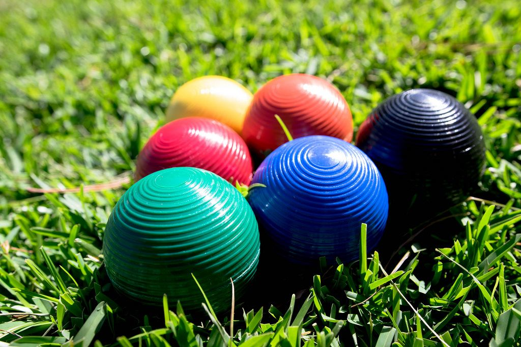
\includegraphics[width=80pt,height=60pt]{C6M04 - DT - Q1i.png}};
\draw (374.5,109.5) node  {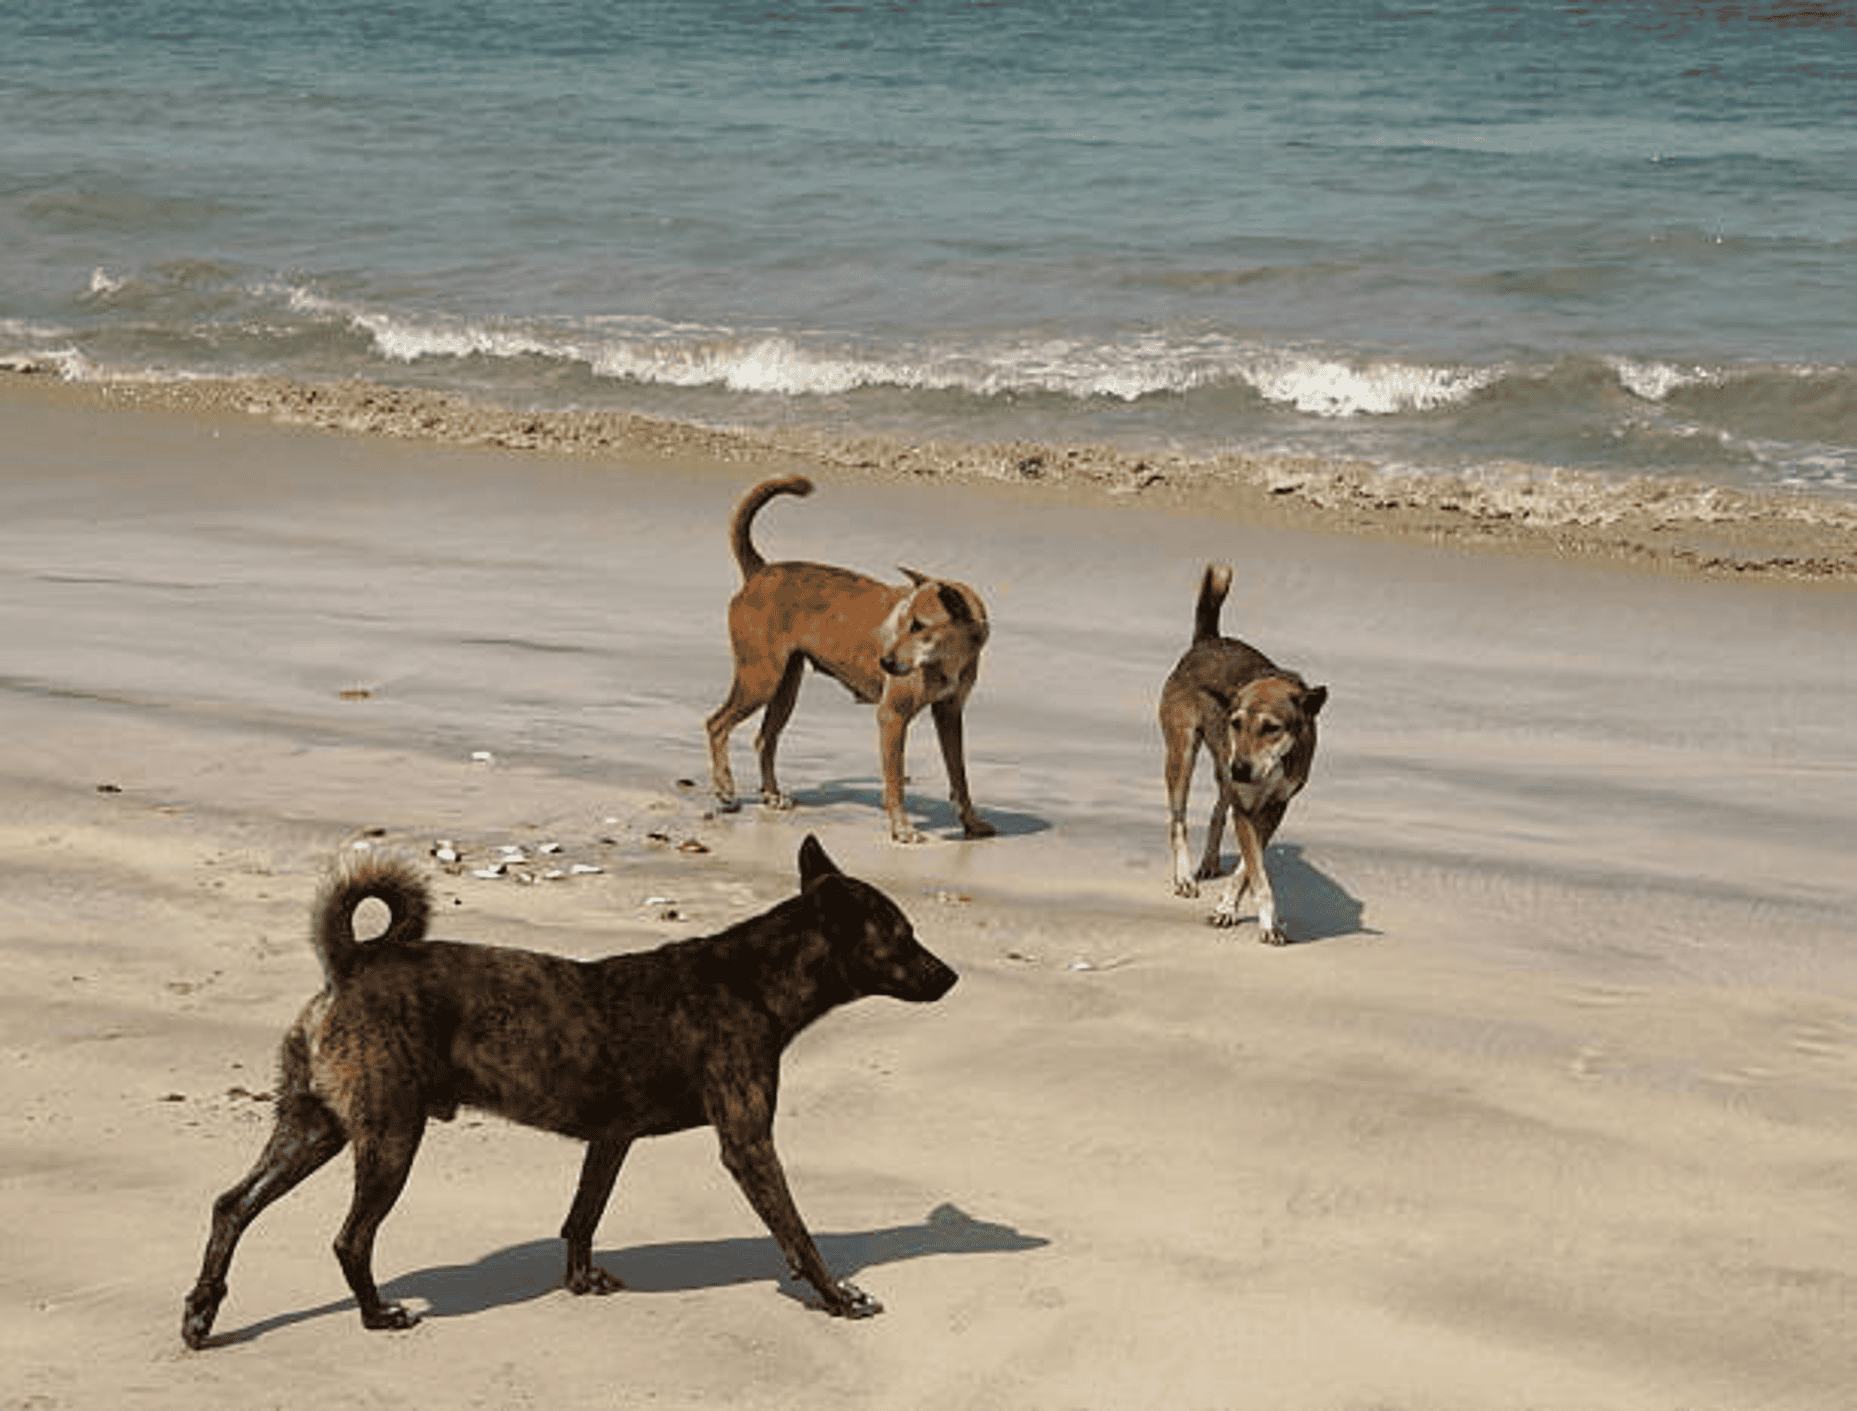
\includegraphics[width=80pt,height=60pt]{C6M04 - DT - Q1ii.png}};
\draw (90,155) node [anchor=north west][inner sep=0.75pt]   [align=left] {Number of balls = \rule{40pt}{0.5pt}};
\draw (295,155) node [anchor=north west][inner sep=0.75pt]   [align=left] {Number of dogs = \rule{40pt}{0.5pt}};
\end{tikzpicture}  
  },
  optionA={Balls},
  optionB={Dogs},
  optionC={Both balls and dogs},
  optionD={None of these},
  questionTag={C6M04 - DT - Q1}, 
  leftmini={0.5},
  rightmini={0.35},
  correctoption={B},
}



\mcqtextbottomOneFour{
  questionnumber={2}, 
  questiontext={Find all the factors of 8.\\
  \smallskip
  \hspace{2cm}
  \colorbox{cyan}{\makebox[1cm][c]{4}} \quad \colorbox{cyan}{\makebox[1cm][c]{1}} \quad
  \colorbox{cyan}{\makebox[1cm][c]{2}} \quad 
  \colorbox{cyan}{\makebox[1cm][c]{6}} \quad 
  \colorbox{cyan}{\makebox[1cm][c]{8}} },
  optionA={1, 2, 8},
  optionB={1, 2, 4, 8},
  optionC={1, 2, 6},
  optionD={4, 6, 8},
  questionTag={C6M04 - DT - Q2}, 
  correctoption={B},
}


\mcqimgleftFourOne{
  questionnumber={6}, 
  questiontext={The given amount is divisible by \rule{40pt}{0.5pt}.},
    imgtabletikz = { 
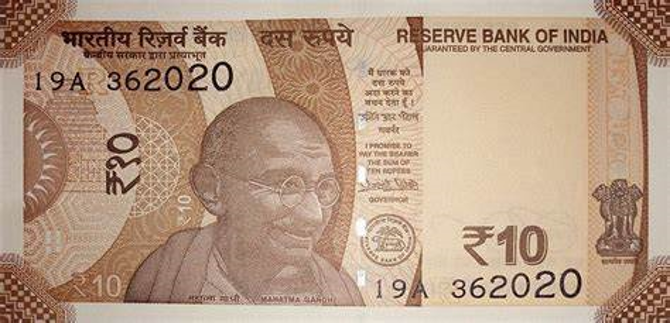
\includegraphics[width=6cm, height=2.5cm]{C6M04 - DT - Q6.png} },
  optionA={5},
  optionB={3},
  optionC={4},
  optionD={6},
  questionTag={C6M04 - DT - Q6}, 
  leftmini={0.4},
  rightmini={0.4},
  correctoption={A},
}


\mcqimgleftFourOne{
  questionnumber={3}, 
  questiontext={The given lines are \rule{80pt}{0.5pt}.},
    imgtabletikz = { 
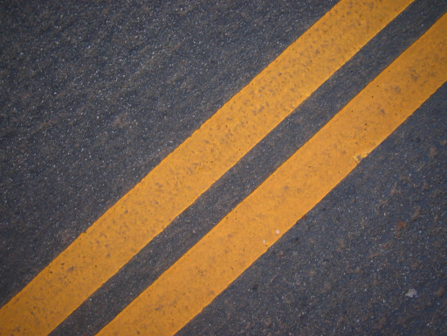
\includegraphics[width=2.5cm, height=2.5cm]{C6M11 - DT - Q3.png} },
  optionA={Perpendicular lines},
  optionB={Intersecting lines},
  optionC={Parallel lines},
  optionD={None of these},
  questionTag={C6M11 - DT - Q3}, 
  correctoption={C},
  leftmini={0.3},
  rightmini={0.6}
}


\mcqtextbottomOneFour{
  questionnumber={4}, 
  questiontext={Which teddy bear shows an incorrect measurement of angles?},
  optionA={ 
\includegraphics[height= 2cm, width=2.8cm]{C6M11 - DT - Q4i.png}  },
  optionB={
\includegraphics[height= 2cm, width=2.8cm]{C6M11 - DT - Q4ii.png}  },
  optionC={
\includegraphics[height= 2cm, width=2.8cm]{C6M11 - DT - Q4iii.png} },
  optionD={ All the above},
  questionTag={C6M11 - DT - Q4}, 
  correctoption={D},
}


\mcqimgleftFourOne{
  questionnumber={1}, 
  questiontext={Name this polygon.},
    imgtabletikz = { 

\includegraphics[width=5cm, height=3cm]{C6M12 - DT - Q1.png} },
  optionA={Square},
  optionB={Heptagon},
  optionC={Octagon},
  optionD={Pentagon},
  questionTag={C6M12 - DT - Q1}, 
  correctoption={C},
  leftmini={0.45},
  rightmini={0.45},
}


\mcqimgleftFourOne{
  questionnumber={2}, 
  questiontext={Identify the colour of the vertices.},
    imgtabletikz = { 
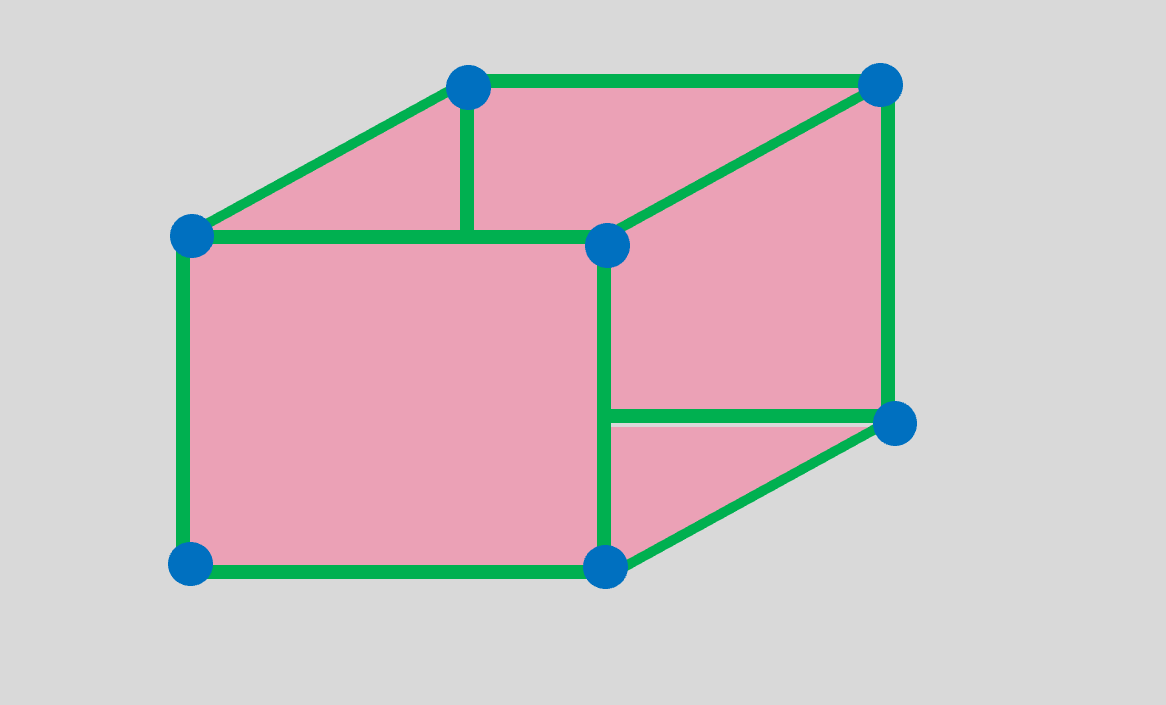
\includegraphics[width=5cm, height=3cm]{C6M13 - DT - Q2.png}},
  optionA={Pink },
  optionB={Blue},
  optionC={Green },
  optionD={Grey},
  questionTag={C6M13 - DT - Q2}, 
  correctoption={B},
  leftmini={0.4},
  rightmini={0.5}
}


\mcqimgleftFourOne{
  questionnumber={1}, 
  questiontext={Represent the given number of ice creams in tallymarks.},
  imgtabletikz = { 

\includegraphics[width=8cm, height=1.5cm]{C6M17 - DT - Q1.png}},
  optionA={
  \tikzset{every picture/.style={line width=0.75pt}} 
\begin{tikzpicture}[x=0.75pt,y=0.75pt,yscale=-0.75,xscale=0.75] 
\draw    (191,100) -- (191,117.8) ; 
\draw    (201.4,100) -- (201.4,117.8) ;
\draw    (195.8,100) -- (195.8,117.8) ; 
\draw    (204,103) -- (189,115.8) ;
\draw    (207.8,100) -- (207.8,117.8) ;
\end{tikzpicture}},
  optionB={
  \tikzset{every picture/.style={line width=0.75pt}} 
\begin{tikzpicture}[x=0.75pt,y=0.75pt,yscale=-0.75,xscale=0.75] 
\draw    (258,101.4) -- (258,119.2) ; 
\draw    (268.4,101.4) -- (268.4,119.2) ;
\draw    (262.8,101.4) -- (262.8,119.2) ;
\draw    (273.2,101.2) -- (273.2,119) ;
\draw    (278.8,101.4) -- (278.8,119.2) ;
\draw    (283.6,101.4) -- (283.6,119.2) ;
\end{tikzpicture}  },
  optionC={ 
\tikzset{every picture/.style={line width=0.75pt}} 
\begin{tikzpicture}[x=0.75pt,y=0.75pt,yscale=-0.75,xscale=0.75]
\draw    (358,82.2) -- (358,100) ;
\draw    (362.8,82.2) -- (362.8,100) ;
\draw    (365.8,83.2) -- (355,97) ;
\draw    (373.2,81.4) -- (373.2,99.2) ; 
\draw    (378,81.4) -- (378,99.2) ; 
\draw    (381,82.4) -- (370.2,96.2) ;
\draw    (389.2,81.4) -- (389.2,99.2) ;
\draw    (394,81.4) -- (394,99.2) ; 
\draw    (397,82.4) -- (386.2,96.2) ;
\draw    (406,82.2) -- (406,100) ; 
\draw    (410.8,82.2) -- (410.8,100) ; 
\draw    (413.8,83.2) -- (403,97) ;
\draw    (422.8,82.2) -- (422.8,100) ;
\draw    (427.6,82.2) -- (427.6,100) ; 
\draw    (430.6,83.2) -- (419.8,97) ;
\draw    (440.4,83) -- (440.4,100.8) ; 
\draw    (445.2,83) -- (445.2,100.8) ;
\draw    (448.2,84) -- (437.4,97.8) ;
\end{tikzpicture} },
  optionD={
\tikzset{every picture/.style={line width=0.75pt}} 
\begin{tikzpicture}[x=0.75pt,y=0.75pt,yscale=-1,xscale=1] 
\draw    (191,100) -- (191,117.8) ; 
\draw    (201.4,100) -- (201.4,117.8) ;
\draw    (195.8,100) -- (195.8,117.8) ; 
\draw    (208.2,102.4) -- (190,119.2) ; 
\draw    (205.8,100) -- (205.8,117.8) ; 
\draw    (212.2,100) -- (212.2,117.8) ;
\end{tikzpicture} },
  questionTag={C6M17 – DT – Q1}, 
  correctoption={D},
  leftmini={0.5},
  rightmini={0.4}
}


\mcqimgleftFourOne{
  questionnumber={3}, 
  questiontext={Find the number of fruits sold on Saturday.},
 imgtabletikz = { 
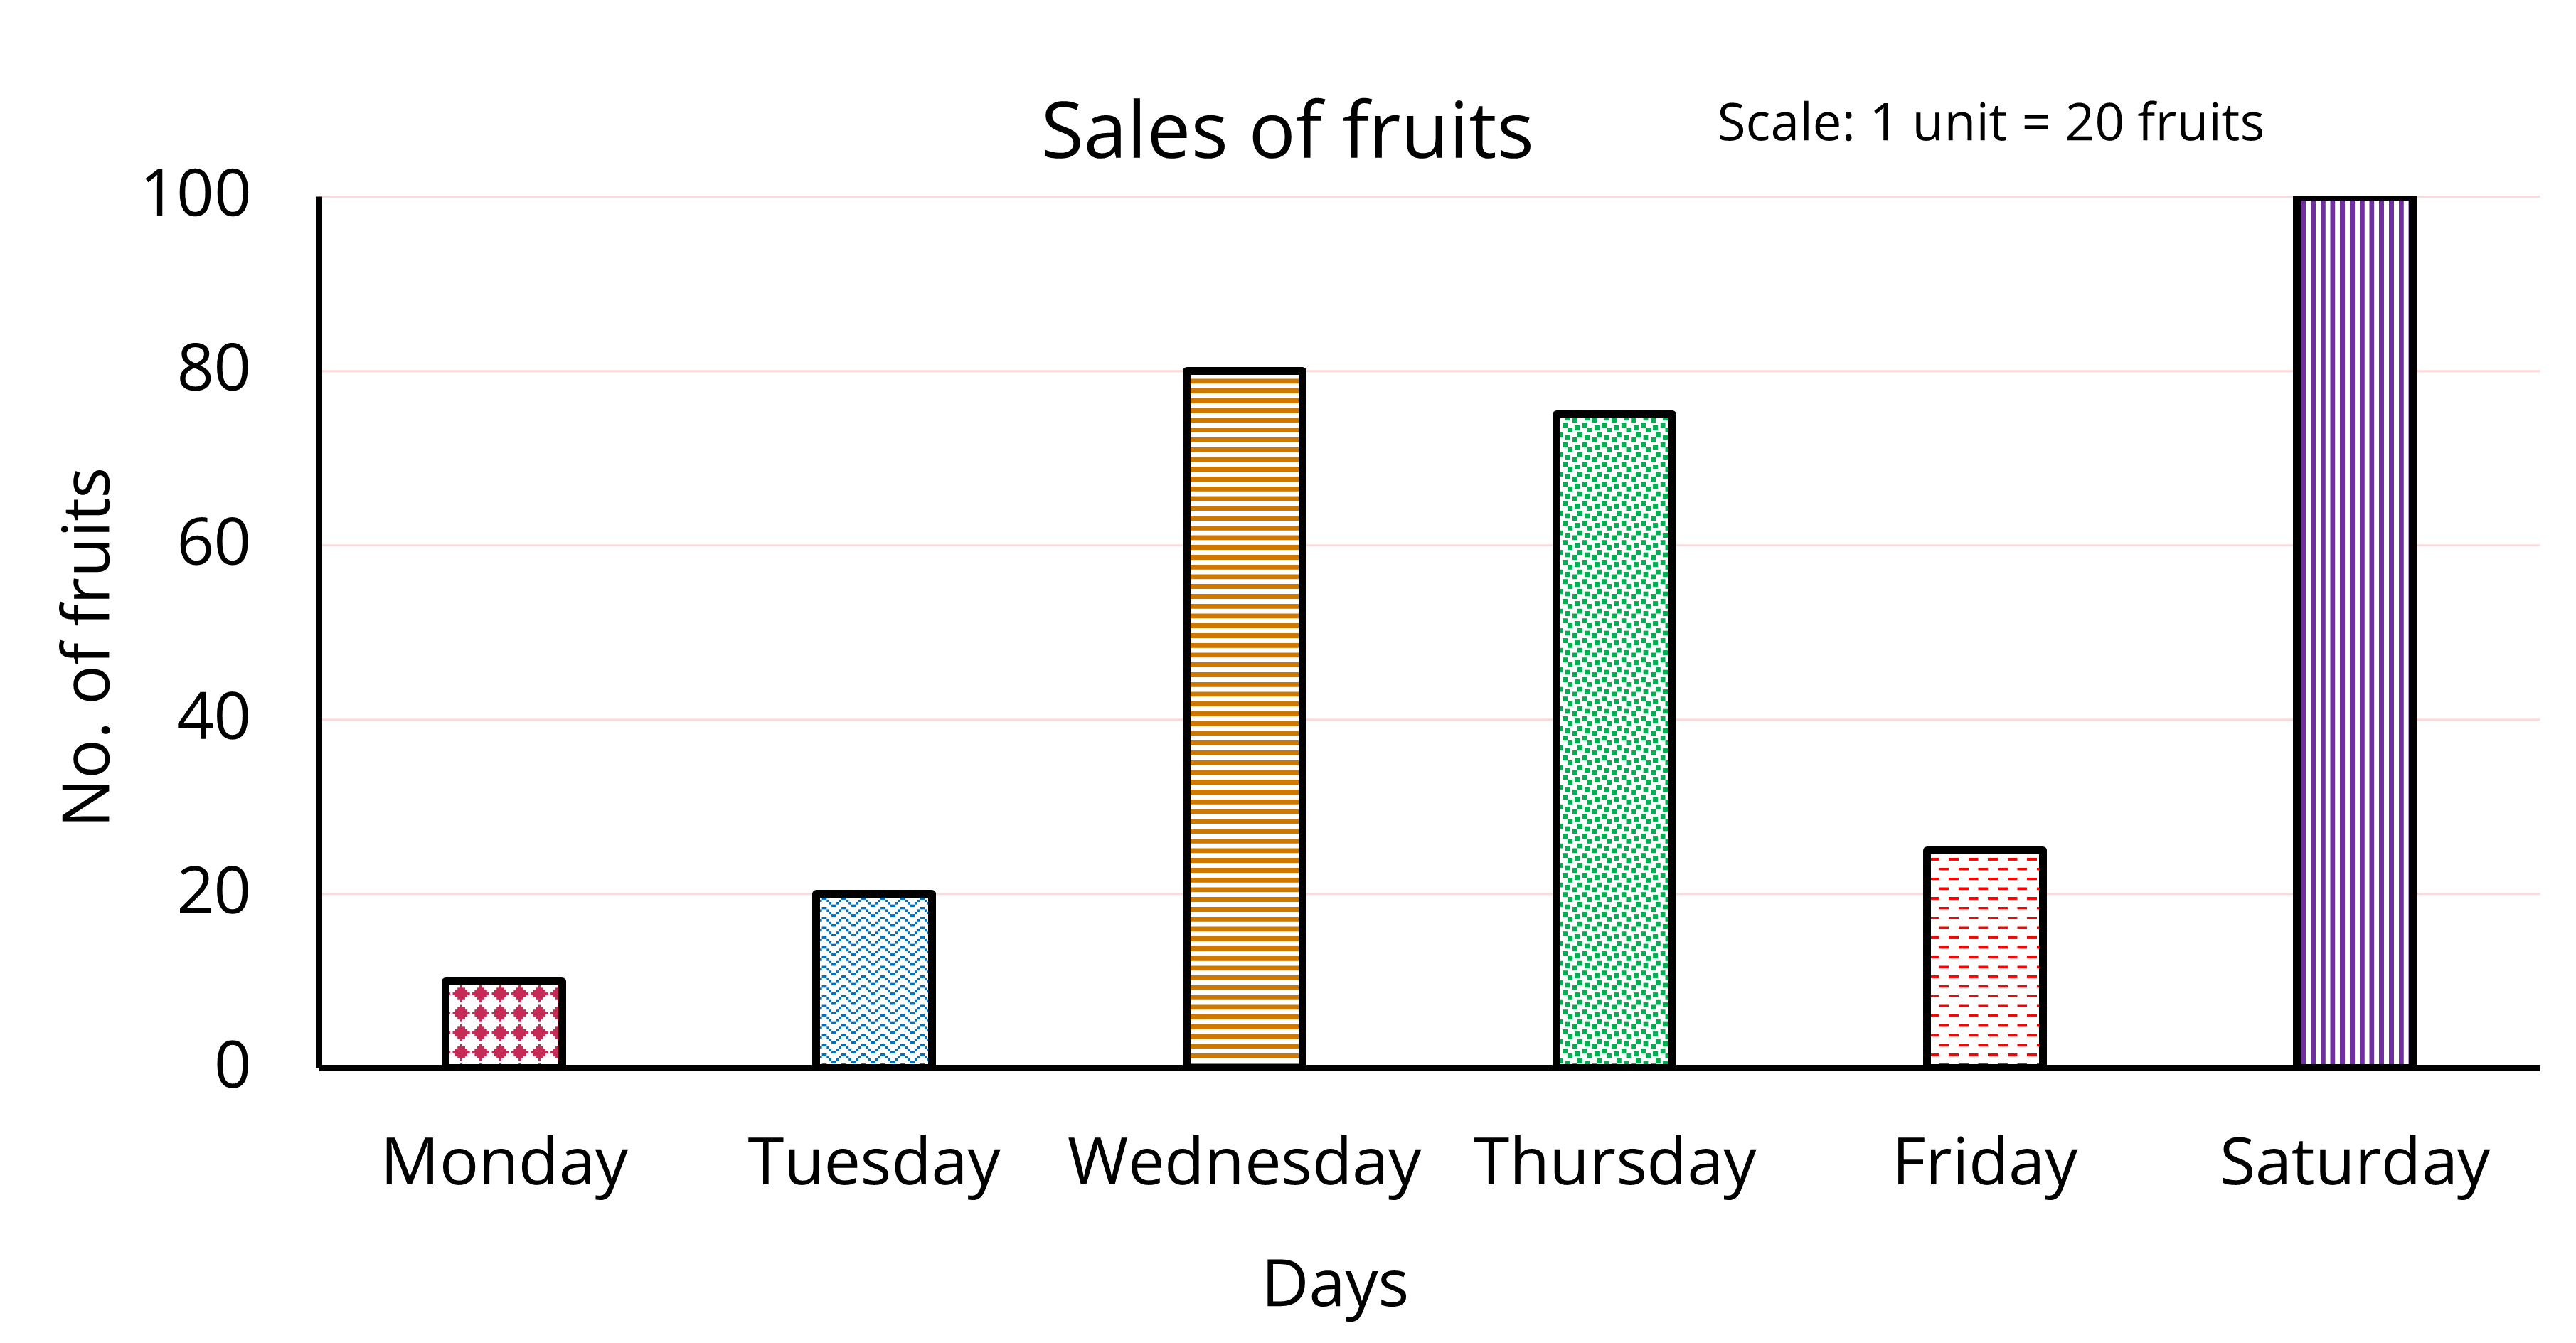
\includegraphics[width=12cm, height=6cm]{C6M17 - DT - Q3.png}},
  optionA={100},
  optionB={80},
  optionC={10},
  optionD={101},
  questionTag={C6M17 – DT – Q3}, 
   leftmini={0.65},
  rightmini={0.25},
  correctoption={A},
}




\mcqimgleftFourOne{
  questionnumber={1}, 
  questionTag={C6M06 – DT – Q1},
  questiontext={If the price of the ball and bat are the same, what will be the lowest common multiple?},
  imgtabletikz  = {
\tikzset{every picture/.style={line width=0.75pt}} 
\begin{tikzpicture}[x=0.75pt,y=0.75pt,yscale=-1,xscale=1]
\draw (223,66.16) node  {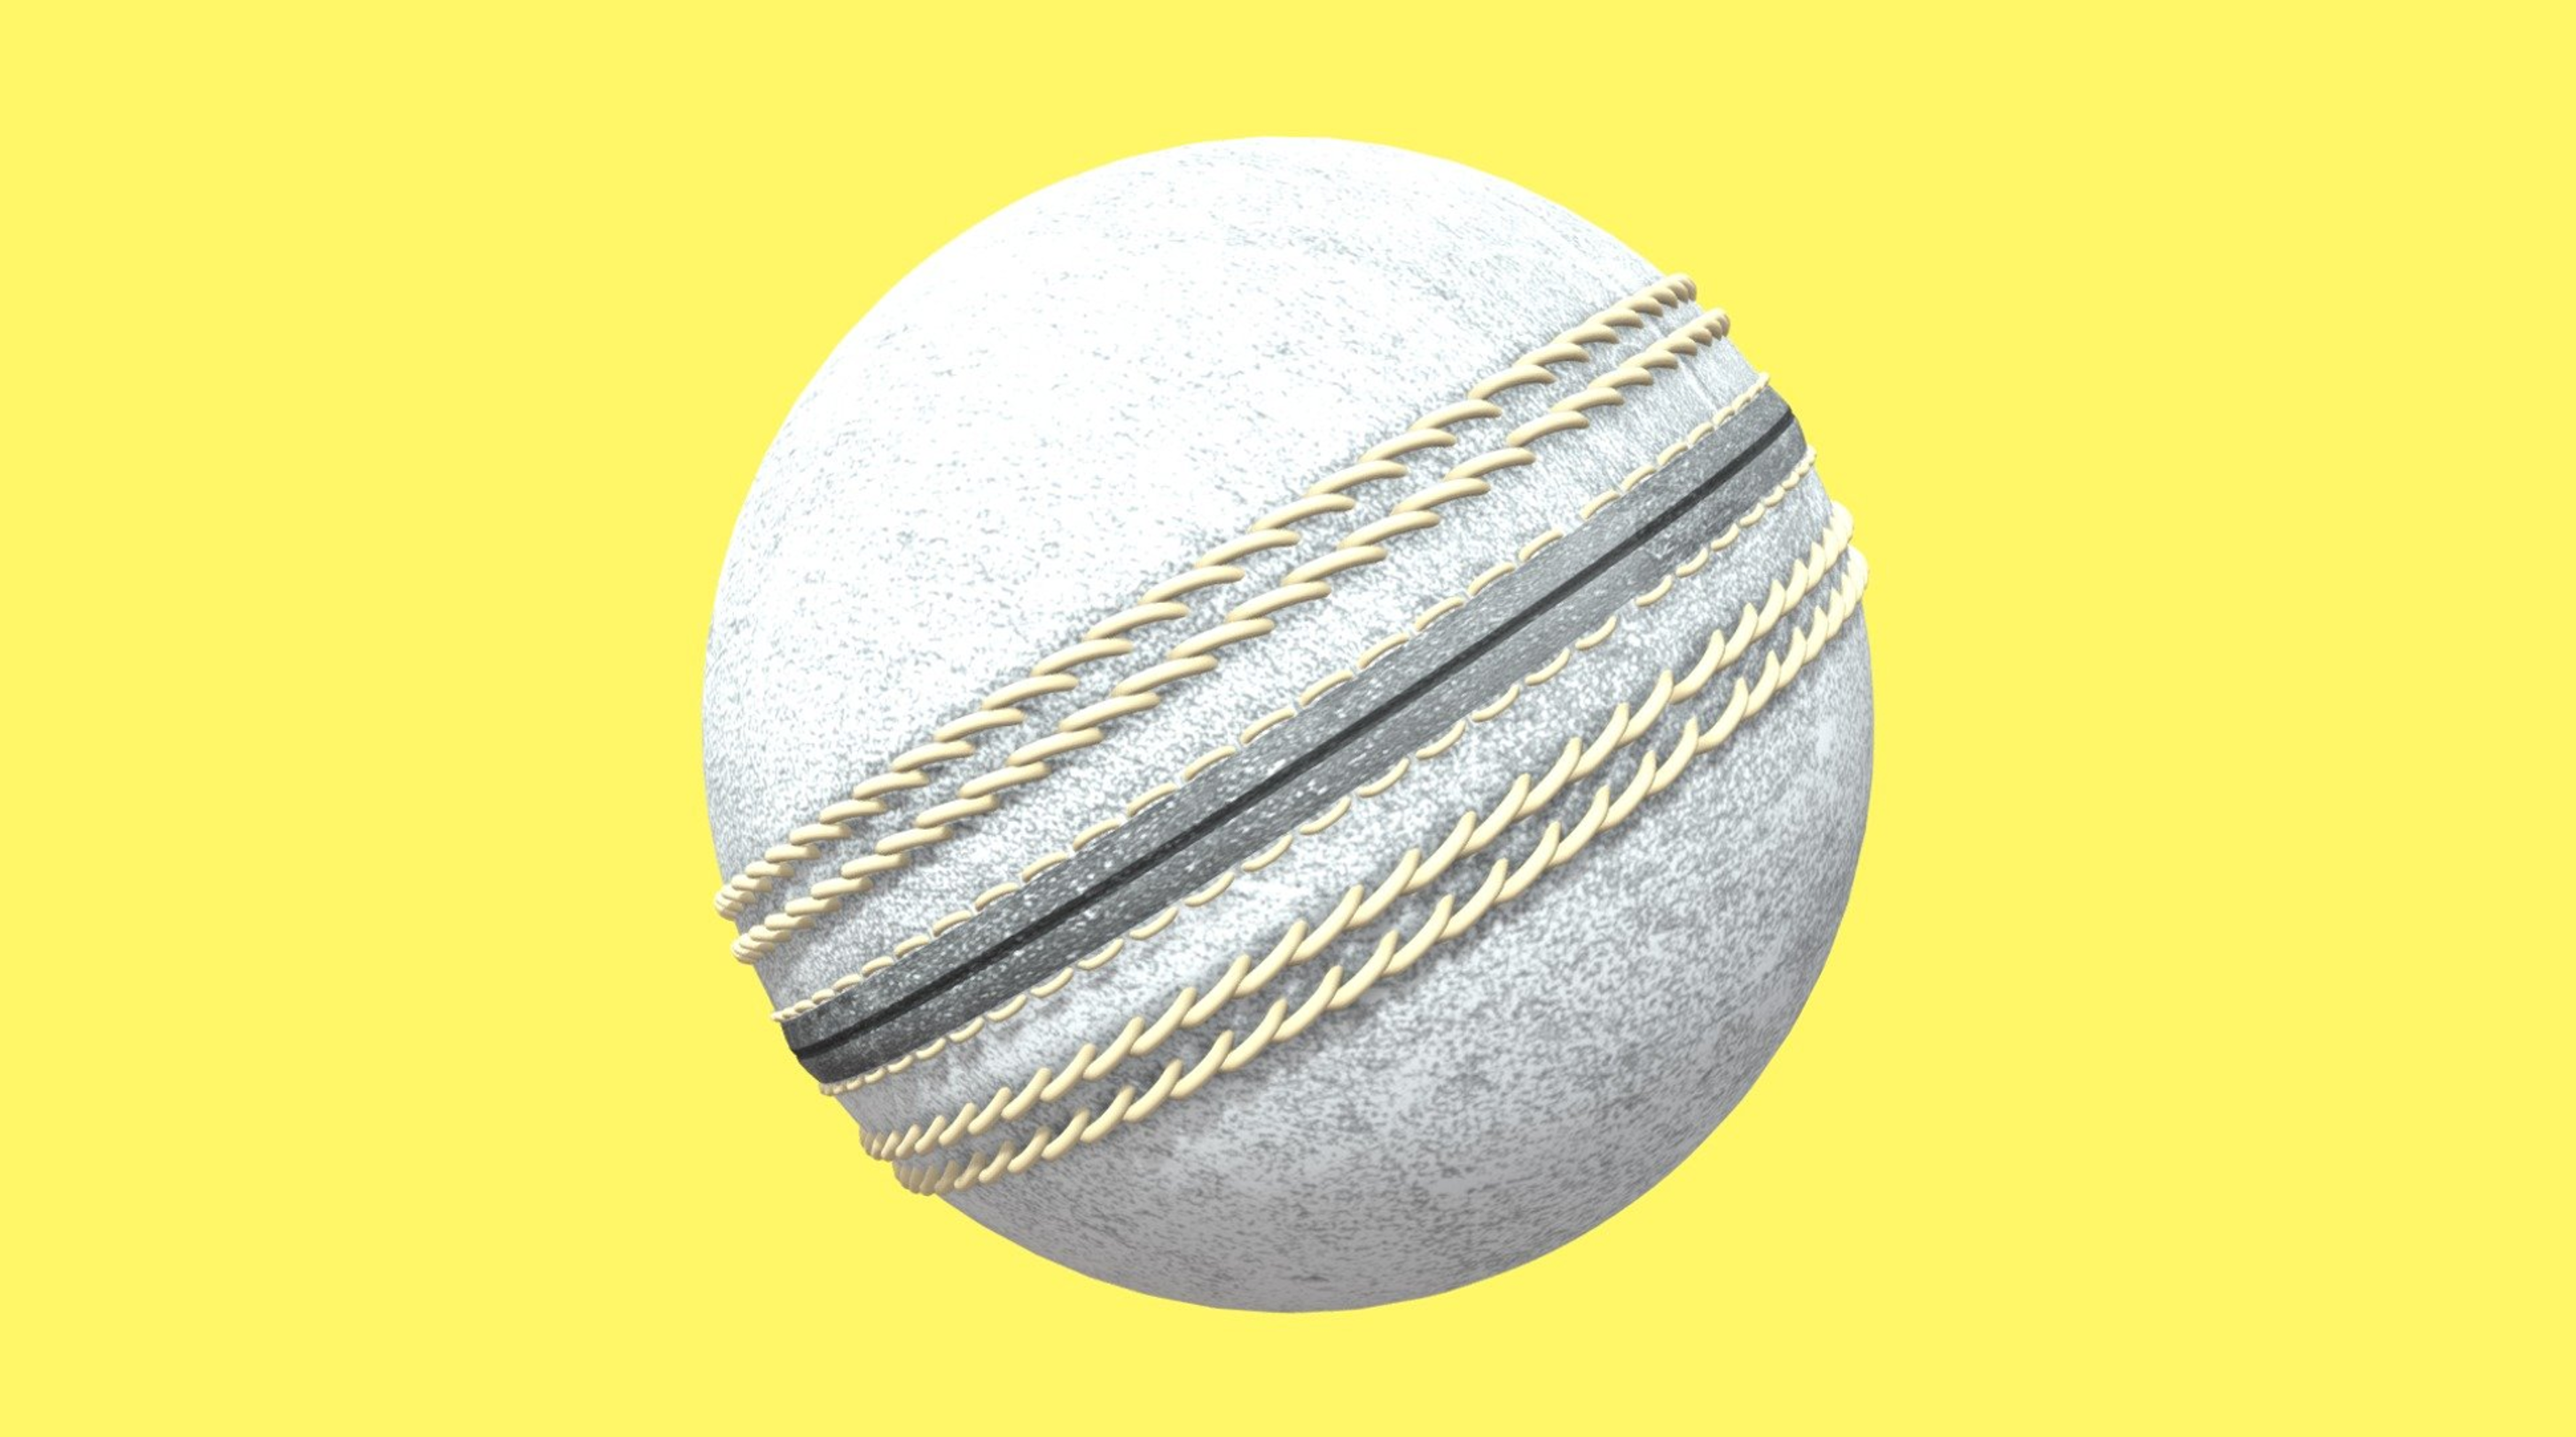
\includegraphics[width=100.5pt,height=57.25pt]{C6M06 - DT - Q1ii.png}};
\draw (410,66.16) node  {
\includegraphics[width=87pt,height=57.25pt]{C6M06 - DT - Q1i.png}};
\draw (195,114) node [anchor=north west][inner sep=0.75pt]   [align=left] {Rs. 120};
\draw (381,110) node [anchor=north west][inner sep=0.75pt]   [align=left] {Rs. 120};
\end{tikzpicture}},
  optionA={240},
  optionB={120},
  optionC={180},
  optionD={60},
  correctoption={B},
  leftmini={0.65},
  rightmini={0.25},
}


\mcqtextbottomOneFour{
  questionnumber={2}, 
  questiontext={Identify the colour of the denominator.\\
\tikzset{every picture/.style={line width=0.75pt}} 
\hspace{5cm}
\begin{tikzpicture}[x=0.75pt,y=0.75pt,yscale=-1,xscale=1]
\draw  [color={rgb, 255:red, 208; green, 2; blue, 27 }  ,draw opacity=1 ][fill={rgb, 255:red, 175; green, 219; blue, 126 }  ,fill opacity=1 ] (176,57) -- (203,57) -- (203,84) -- (176,84) -- cycle ;
\draw [color={rgb, 255:red, 208; green, 2; blue, 27 }  ,draw opacity=1 ]   (167,88) -- (214,88) ;
\draw  [color={rgb, 255:red, 208; green, 2; blue, 27 }  ,draw opacity=1 ][fill={rgb, 255:red, 248; green, 240; blue, 140 }  ,fill opacity=1 ] (176,93) -- (203,93) -- (203,120) -- (176,120) -- cycle ;
\draw (184,63) node [anchor=north west][inner sep=0.75pt]   [align=left] {5};
\draw (184,99) node [anchor=north west][inner sep=0.75pt]   [align=left] {4};
\end{tikzpicture} },
  optionA={Yellow},
  optionB={Green},
  optionC={Red},
  optionD={Green, Yellow},
  questionTag={C6M06 - DT - Q2}, 
  correctoption={A},
}



\mcqtextbottomOneFour{
  questionnumber={3}, 
  questiontext={Write the fraction of the raw mango from the given image.\\
  \hspace{3cm}
  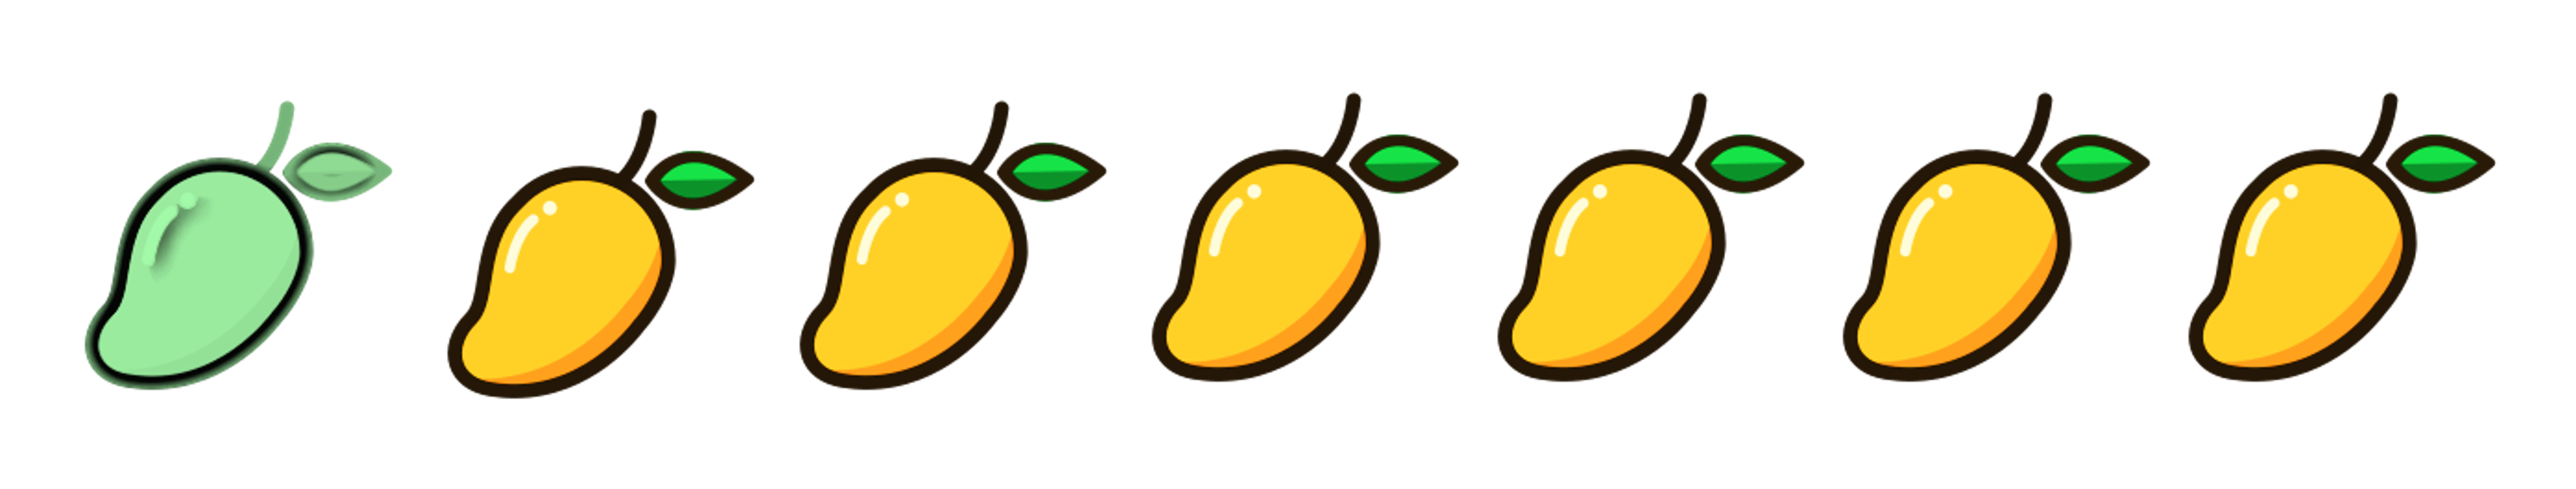
\includegraphics[width=10cm, height = 1.5cm]{C6M06 - DT - Q3.png}},
  optionA={  {\large{$\frac{1}{6}$}}},
  optionB={ {\large{$\frac{7}{10}$}} },
  optionC={ {\large{$\frac{1}{7}$}} },
  optionD={ {\large{$\frac{6}{7}$}} },
  questionTag={C6M06 – DT – Q3}, 
  correctoption={C},
}

\mcqimgleftFourOne{
  questionnumber={9}, 
  questiontext={Compare the fractions of the remaining pizza slices.},
  imgtabletikz = { 
\tikzset{every picture/.style={line width=0.75pt}} 
\begin{tikzpicture}[x=0.75pt,y=0.75pt,yscale=-1,xscale=1]
\draw (221.5,75.5) node  {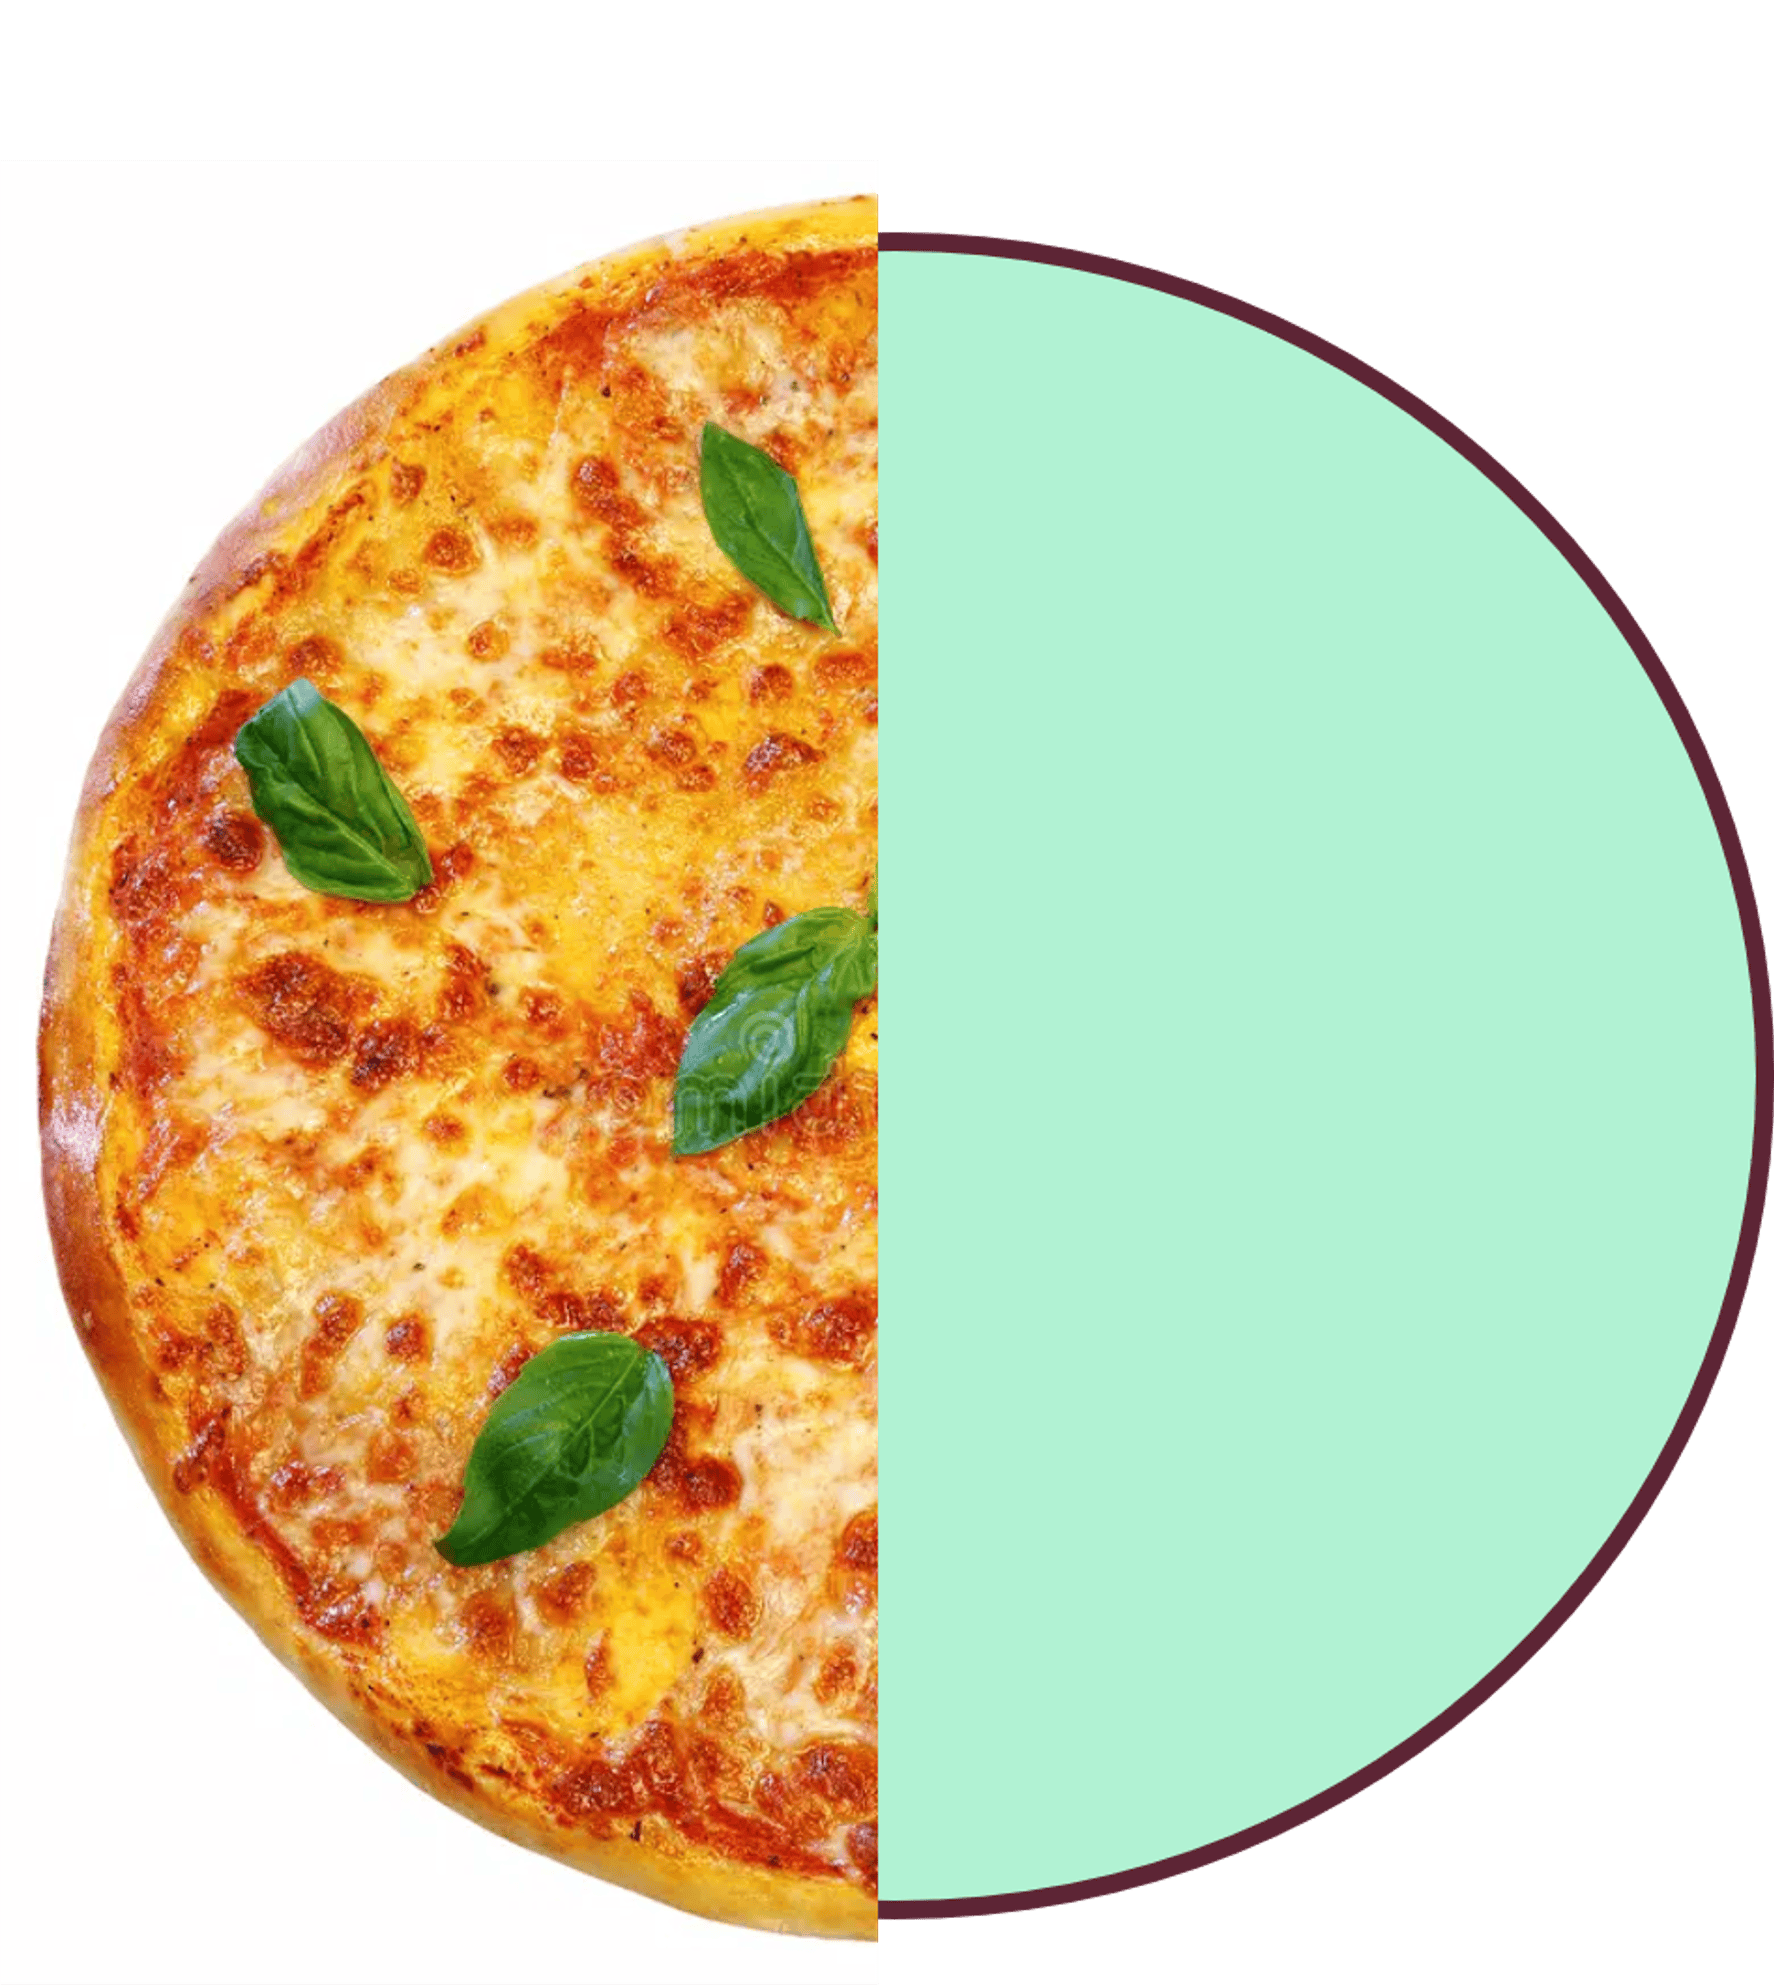
\includegraphics[width=75.75pt,height=75.75pt]{C6M06 - DT - Q9ii.png}};
\draw   (306,62) -- (339,62) -- (339,95) -- (306,95) -- cycle ;
\draw (419.5,75.5) node  {
\includegraphics[width=85pt,height=73pt]{C6M06 - DT - Q9i.png}};
\end{tikzpicture}
  },
   optionA={$>$},
  optionB={$=$},
  optionC={$<$},
  optionD={Undefined},
  questionTag={C6M06 – DT – Q9}, 
  leftmini={0.5},
  rightmini={0.4}, 
  correctoption={C},
}


\mcqimgleftFourOne{
  questionnumber={2}, 
  questionTag={C6M07 - DT - Q2}, 
  questiontext={How much weight should be applied on the other side of the kid in the seesaw to lift him above?},
    imgtabletikz = { 
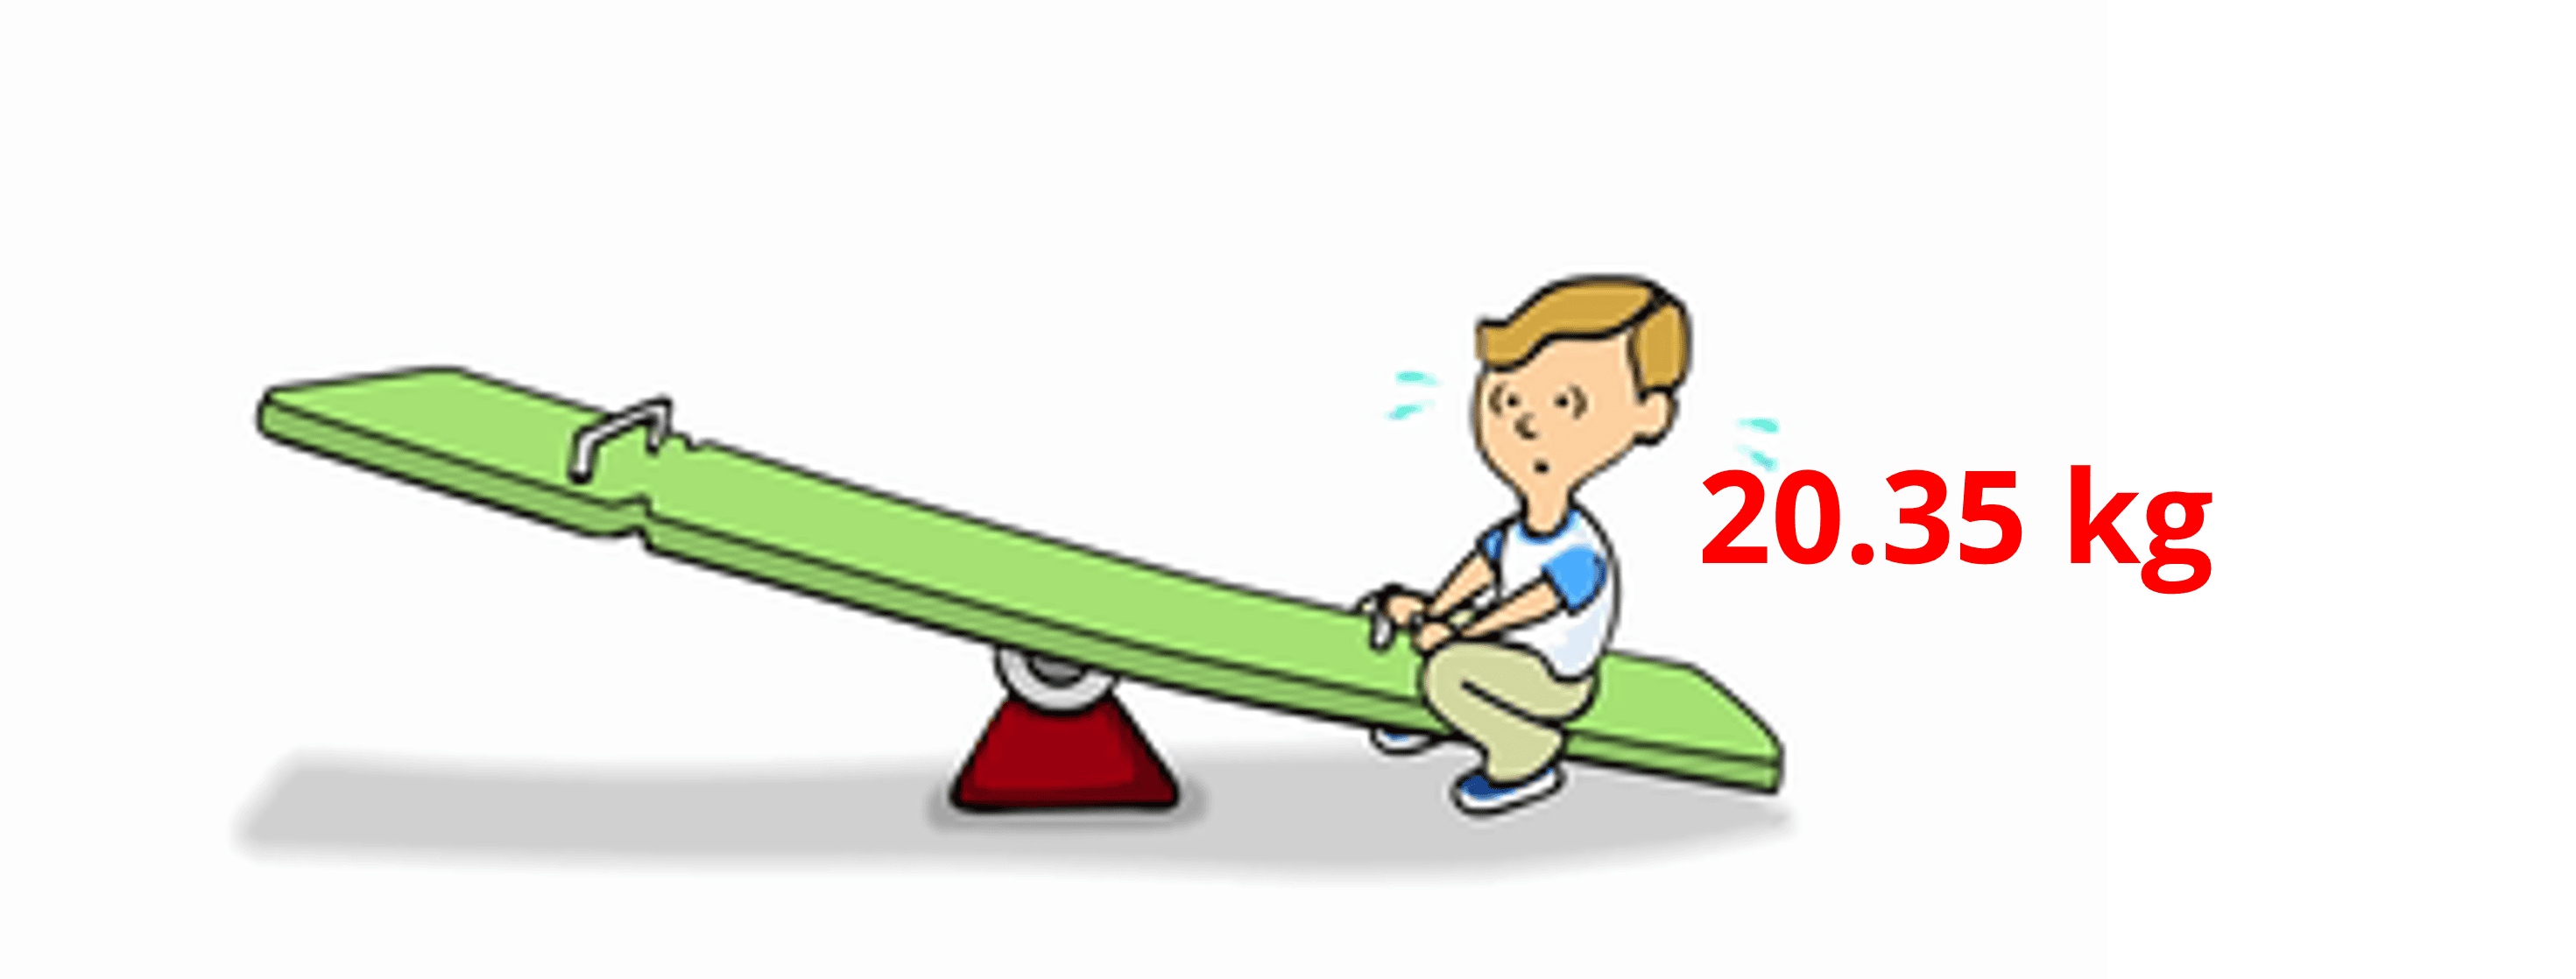
\includegraphics[width=9cm, height=3cm]{C6M07 - DT - Q2.png}   },
  optionA={20.25 kg},
  optionB={20.05 kg},
  optionC={20.75 kg},
  optionD={20.100 kg},
  correctoption={C},
  leftmini={0.6},
  rightmini={0.8},
}


\mcqimgleftFourOne{
  questionnumber={4}, 
  questionTag={C6M07 - DT - Q4},
 questiontext={Find the man‘s height in cm.},
 imgtabletikz  = { 
\tikzset{every picture/.style={line width=0.75pt}} 
\begin{tikzpicture}[x=0.75pt,y=0.75pt,yscale=-1,xscale=1]
\draw    (158.17,20.61) -- (158.71,122.62) ;
\draw [shift={(158.73,125.62)}, rotate = 269.69] [fill={rgb, 255:red, 0; green, 0; blue, 0 }  ][line width=0.08]  [draw opacity=0] (8.93,-4.29) -- (0,0) -- (8.93,4.29) -- cycle    ;
\draw [shift={(158.15,17.61)}, rotate = 89.69] [fill={rgb, 255:red, 0; green, 0; blue, 0 }  ][line width=0.08]  [draw opacity=0] (8.93,-4.29) -- (0,0) -- (8.93,4.29) -- cycle    ;
\draw (129.64,73.42) node  {
\includegraphics[width=27.96pt,height=87.57pt]{C6M07 - DT - Q4.png}};
\draw (159.49,62.28) node [anchor=north west][inner sep=0.75pt]   [align=left] {\textbf{1.5 m}};
\end{tikzpicture} },
  optionA={1.5 cm},
  optionB={15 cm},
  optionC={150 cm},
  optionD={5100 cm},
  correctoption={C},
  leftmini={0.65},
  rightmini={0.35},
}


\mcqimgleftFourOne{
  questionnumber={4}, 
  questionTag={C6M16 - DT - Q4}, 
  questiontext={Find the area of the given rectangular notebook.},
  imgtabletikz  = {
\tikzset{every picture/.style={line width=0.75pt}} 
\begin{tikzpicture}[x=0.75pt,y=0.75pt,yscale=-1,xscale=1]
\draw (244.25,113.49) node  {
\includegraphics[width=81.38pt,height=95.24pt]{C6M16 - DT - Q4.png}};
\draw [line width=1.5]    (303.41,66.12) -- (302.75,165.15) ;
\draw [shift={(302.73,169.15)}, rotate = 270.38] [fill={rgb, 255:red, 0; green, 0; blue, 0 }  ][line width=0.08]  [draw opacity=0] (11.61,-5.58) -- (0,0) -- (11.61,5.58) -- cycle    ;
\draw [shift={(303.43,62.12)}, rotate = 90.38] [fill={rgb, 255:red, 0; green, 0; blue, 0 }  ][line width=0.08]  [draw opacity=0] (11.61,-5.58) -- (0,0) -- (11.61,5.58) -- cycle    ;
\draw [line width=1.5]    (288.16,183.81) -- (208.8,183.17) ;
\draw [shift={(204.8,183.14)}, rotate = 0.46] [fill={rgb, 255:red, 0; green, 0; blue, 0 }  ][line width=0.08]  [draw opacity=0] (11.61,-5.58) -- (0,0) -- (11.61,5.58) -- cycle    ;
\draw [shift={(292.16,183.84)}, rotate = 180.46] [fill={rgb, 255:red, 0; green, 0; blue, 0 }  ][line width=0.08]  [draw opacity=0] (11.61,-5.58) -- (0,0) -- (11.61,5.58) -- cycle    ;
\draw (307.65,109.71) node [anchor=north west][inner sep=0.75pt]   [align=left] {45 cm};
\draw (224.51,190.15) node [anchor=north west][inner sep=0.75pt]   [align=left] {31 cm};
\end{tikzpicture} },
 optionA={ $1395$ cm},
  optionB={$2025$ cm},
  optionC={$1395$ sq. cm},
  optionD={$2025$ sq. cm},
  correctoption={C},
  leftmini={0.5},
  rightmini={0.4},
}

\mcqimgleftFourOne{
  questionnumber={2}, 
  questionTag={C6M14 - DT - Q2}, 
  questiontext={Find the number of lines of symmetry for the given image.},
    imgtabletikz = { 
\includegraphics[width=4cm, height=3cm]{C6M14 - DT - Q2.png}  },
  optionA={Zero},
  optionB={Two},
  optionC={Three},
  optionD={One},
  correctoption={D},
  leftmini={0.5},
  rightmini={0.4},}



\mcqtextbottomOneFour{
  questionnumber={3}, 
  questionTag={C6M14 - DT - Q3}, 
  questiontext={Find the correct reflection of the given image.\\
  \medskip
\tikzset{every picture/.style={line width=0.75pt}} 
\hspace{3cm}
\begin{tikzpicture}[x=0.75pt,y=0.75pt,yscale=-1,xscale=1]
\draw (220.5,127.5) node  {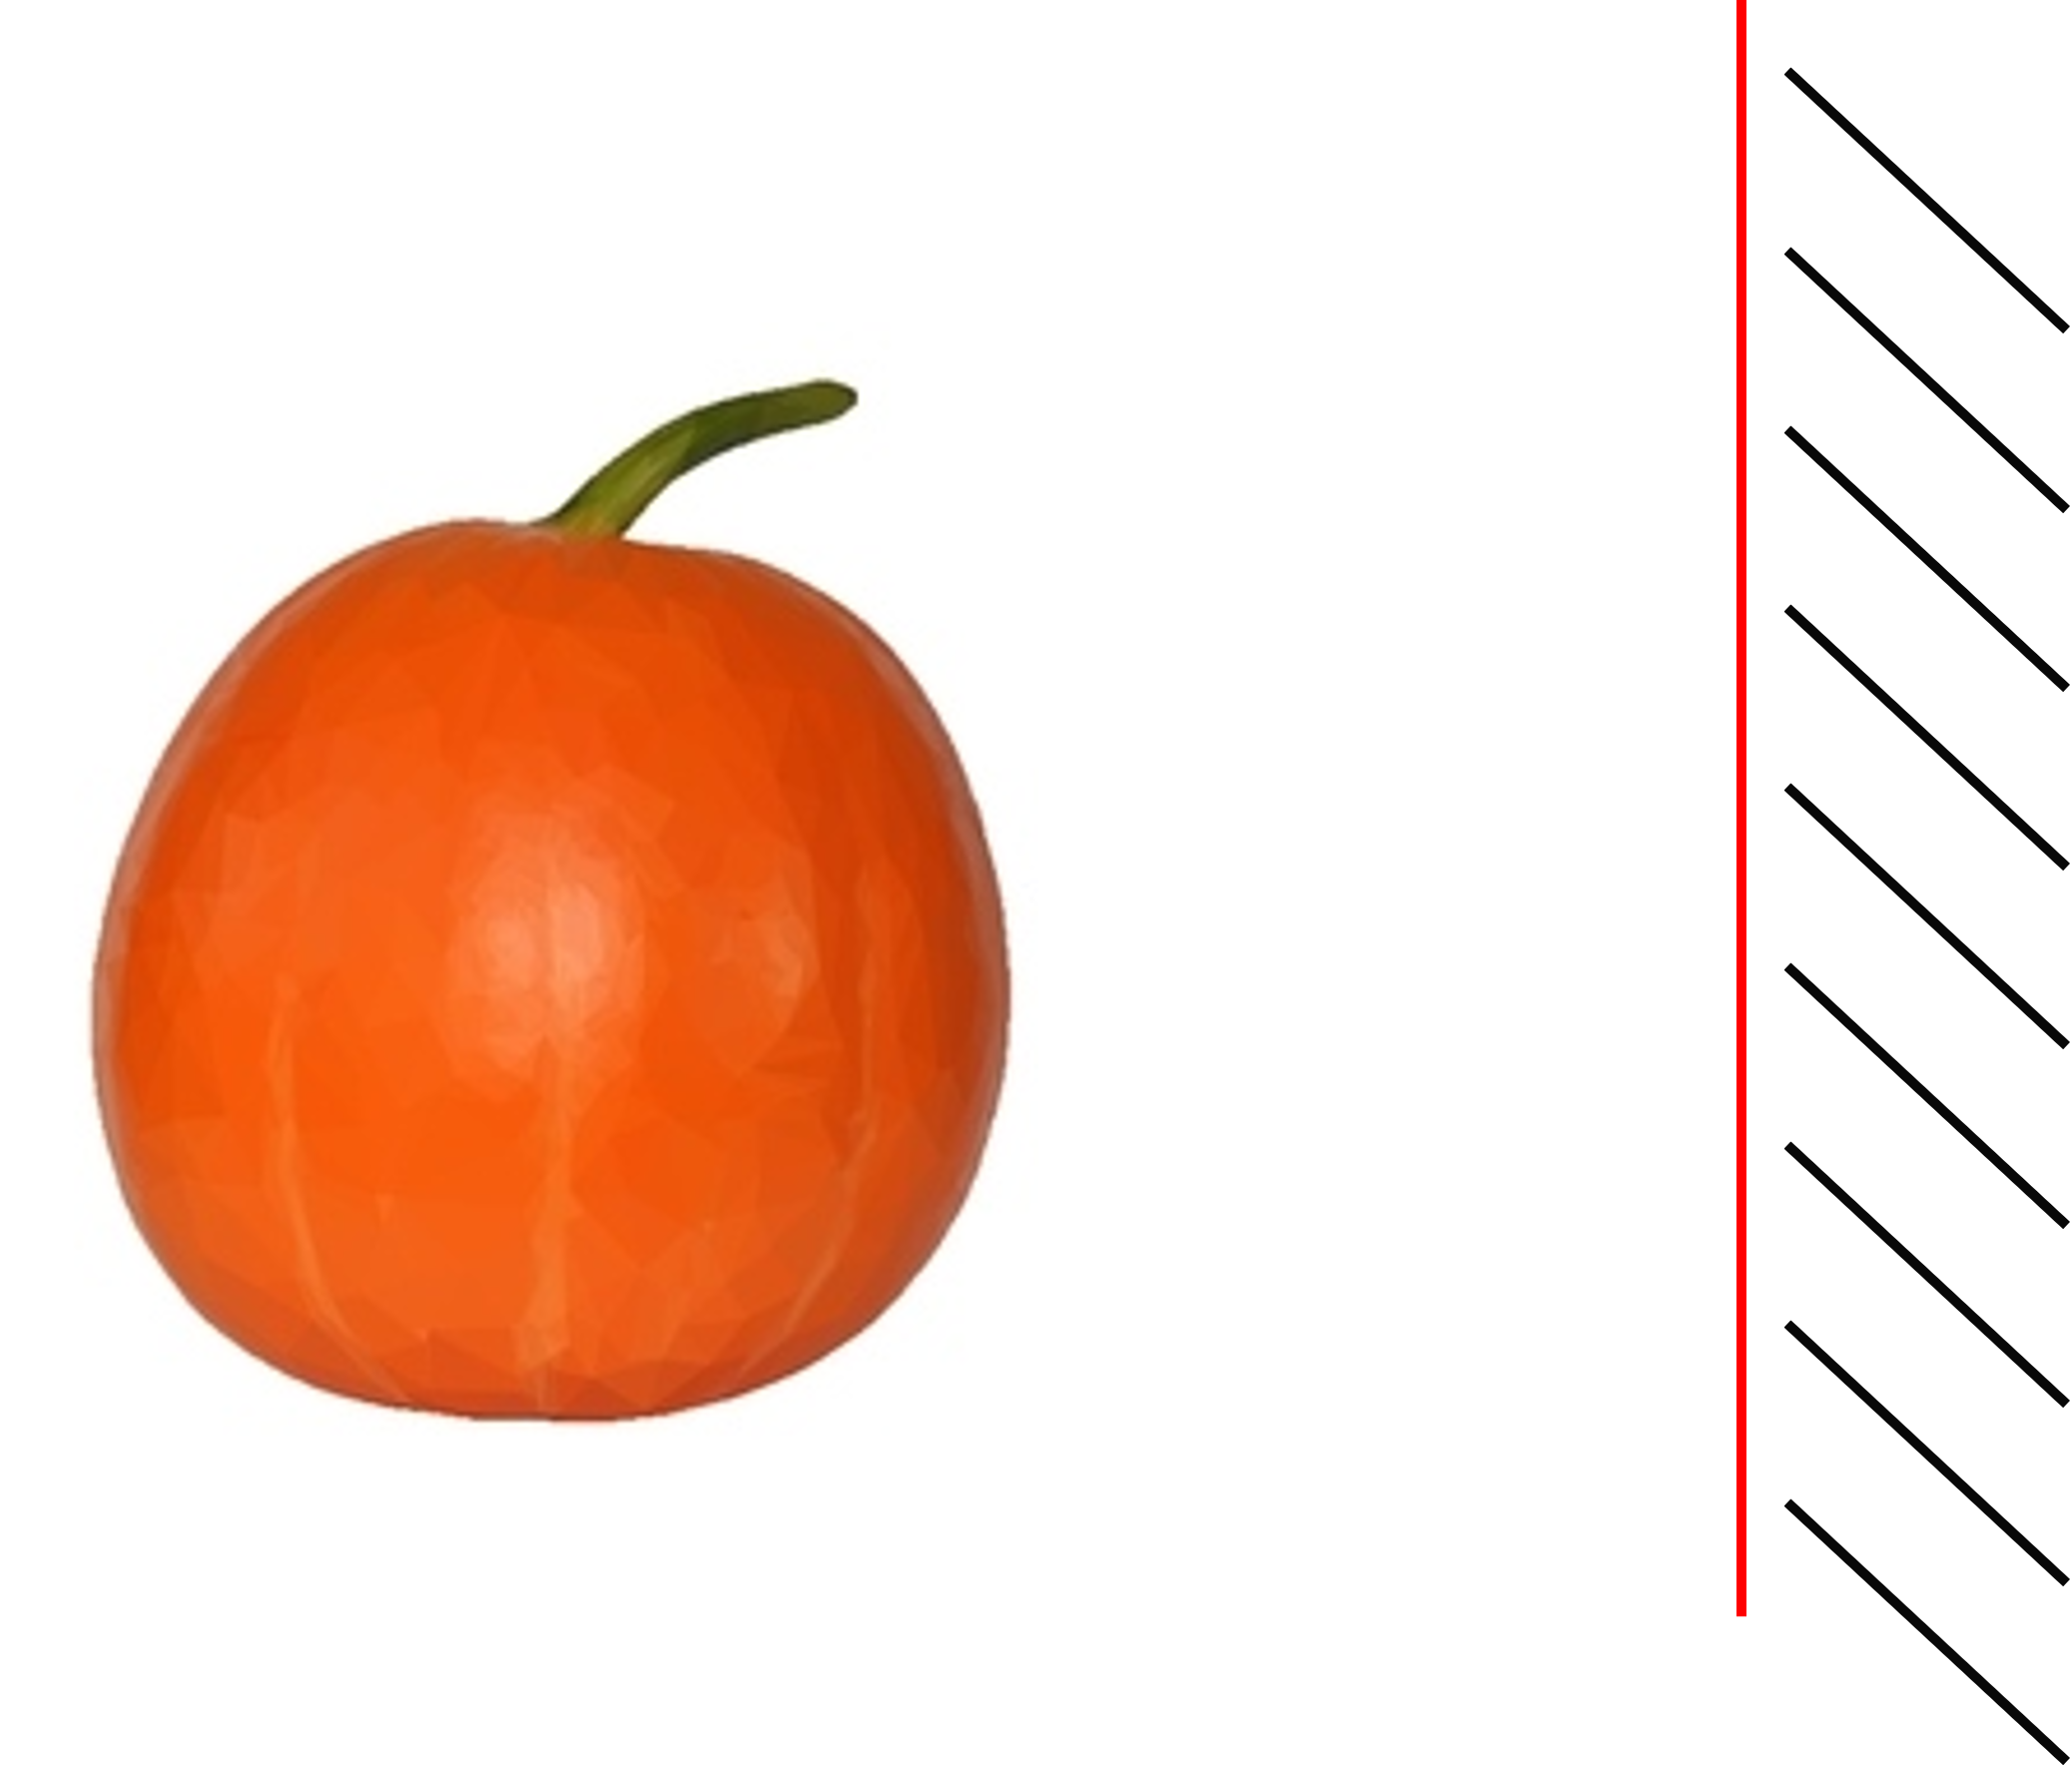
\includegraphics[width=119.25pt,height=95.25pt]{C6M14 - DT - Q3.png}};
\draw (256,38) node [anchor=north west][inner sep=0.75pt]   [align=left] {Mirror};
\end{tikzpicture} },
  optionA={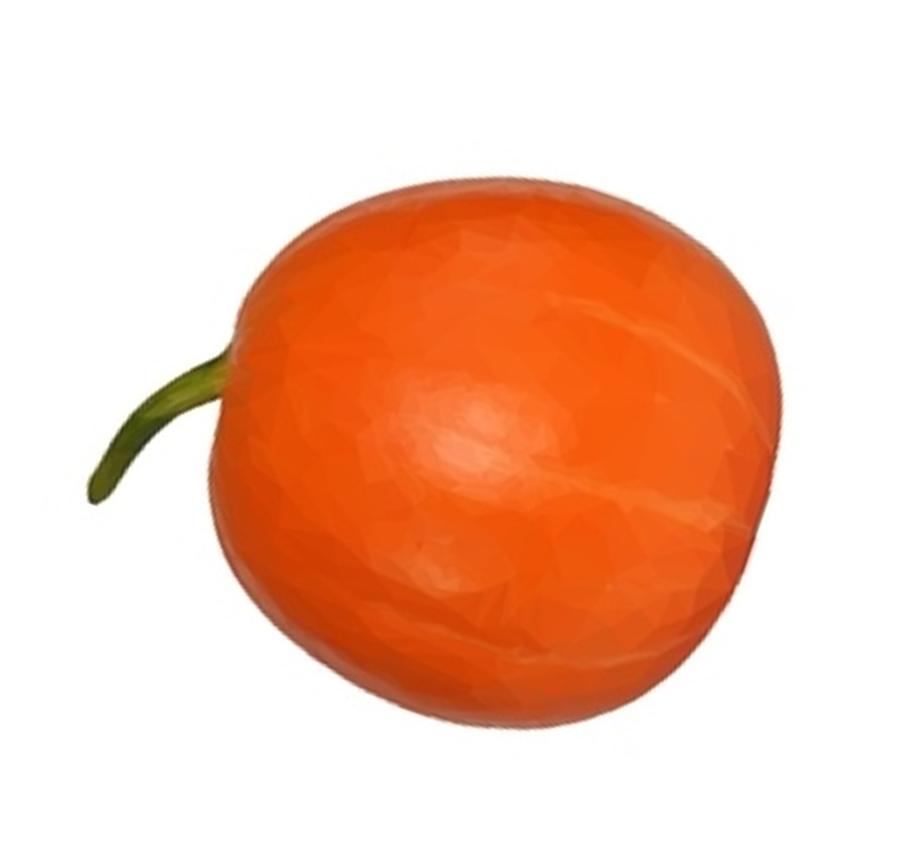
\includegraphics[width=70pt,height=50pt]{C6M14 - DT - Q3i.png}},
  optionB={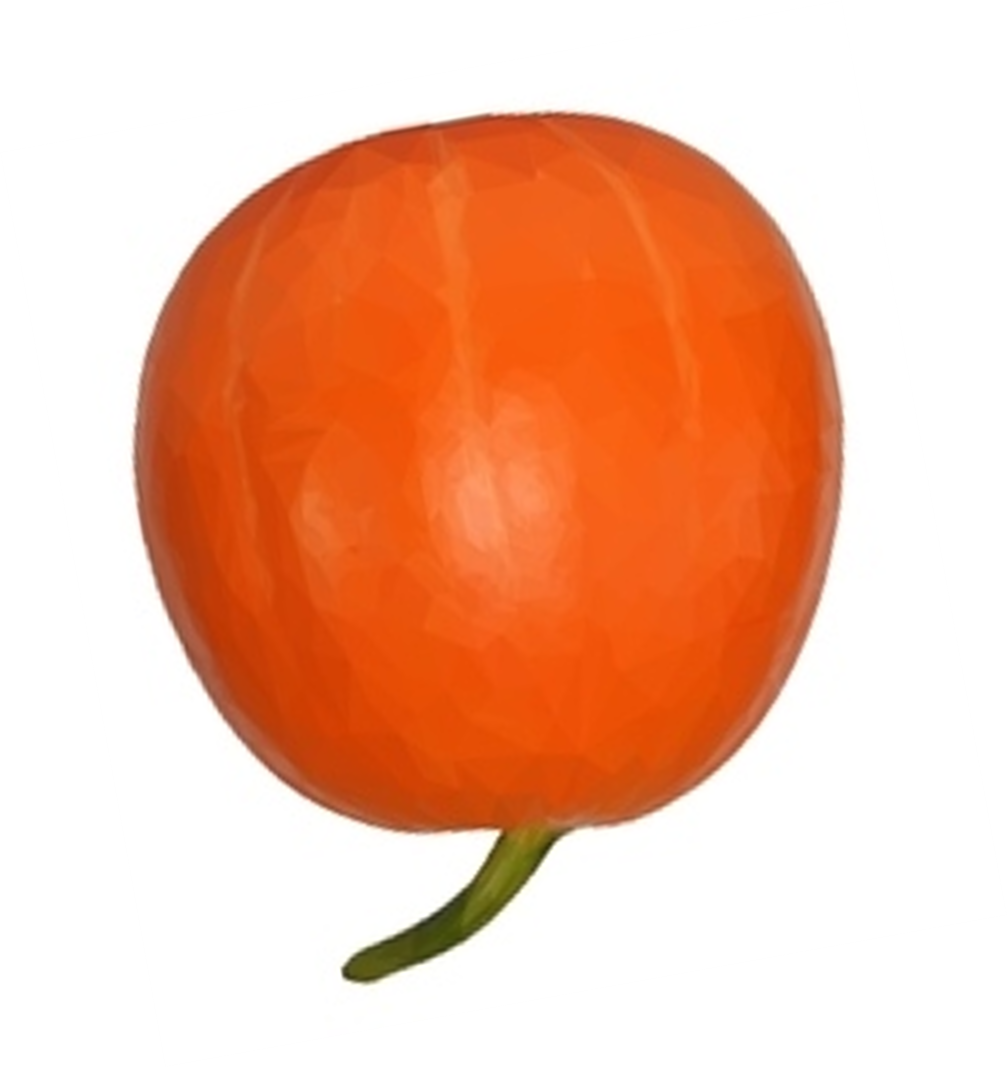
\includegraphics[width=70pt,height=50pt]{C6M14 - DT - Q3ii.png}},
  optionC={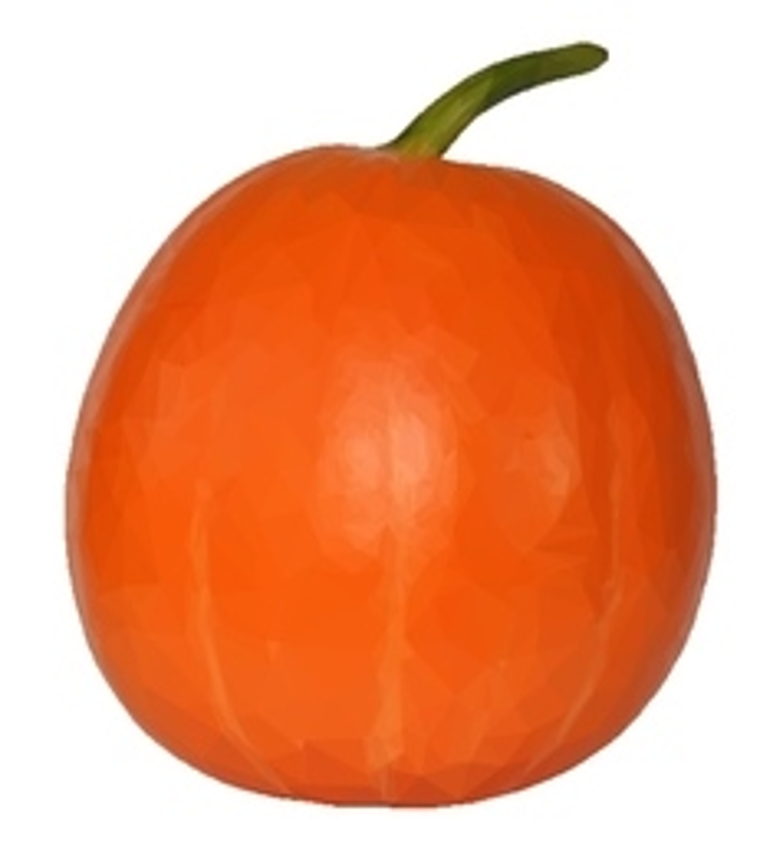
\includegraphics[width=70pt,height=50pt]{C6M14 - DT - Q3iii.png}},
  optionD={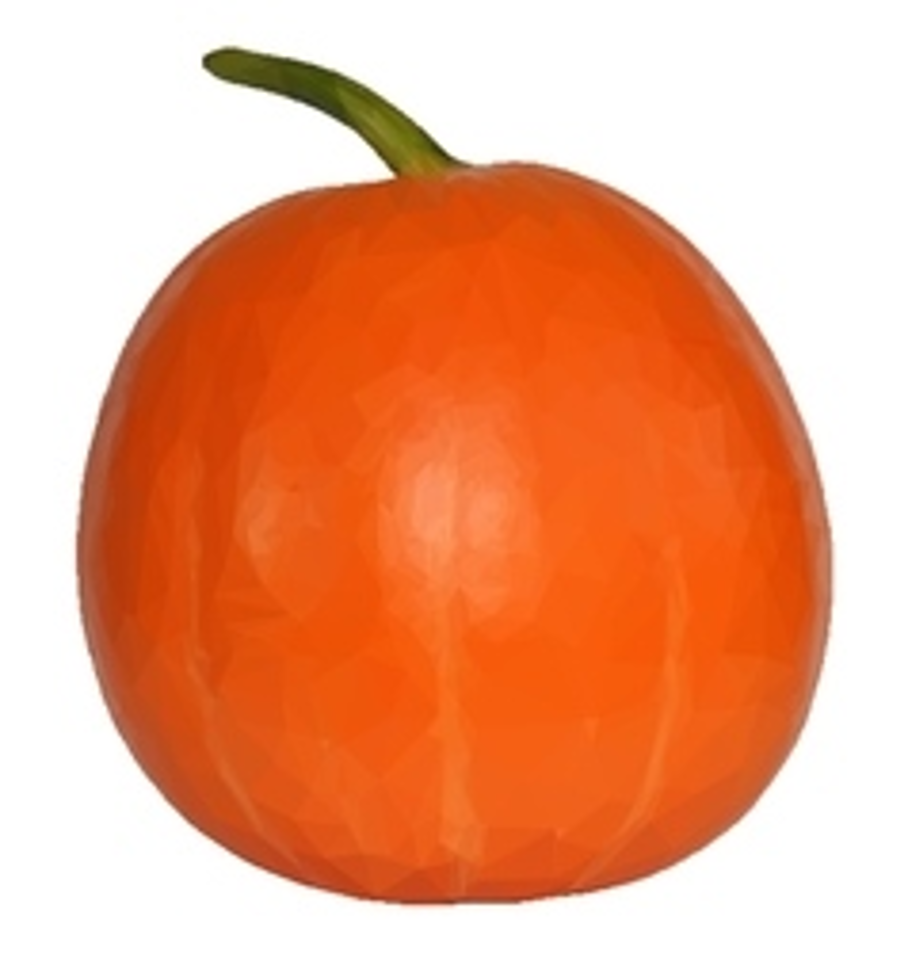
\includegraphics[width=70pt,height=50pt]{C6M14 - DT - Q3iv.png}},
  correctoption={D},}




\mcqtextbottomOneFour{
  questionnumber={1}, 
  questionTag={C5BM - BM - Q1}, 
  questiontext={Add the following.\\
  \begin{table}[H]
      \centering
      \begin{tabular}{ccccc}
           
\includegraphics[width=1.5cm,height=1cm]{C5BM - BM - Q1.png} 
\includegraphics[width=1.5cm,height=1cm]{C5BM - BM - Q1.png} 
\includegraphics[width=1.5cm,height=1cm]{C5BM - BM - Q1.png} & \multirow{2}{*}{+} & 
\includegraphics[width=1.5cm,height=1cm]{C5BM - BM - Q1.png} 
\includegraphics[width=1.5cm,height=1cm]{C5BM - BM - Q1.png} 
\includegraphics[width=1.5cm,height=1cm]{C5BM - BM - Q1.png} 
\includegraphics[width=1.5cm,height=1cm]{C5BM - BM - Q1.png} & \multirow{2}{*}{=} & \multirow{2}{*}{\rule{50pt}{0.5pt}}  \\ 
            
\includegraphics[width=1.5cm,height=1cm]{C5BM - BM - Q1.png} 
\includegraphics[width=1.5cm,height=1cm]{C5BM - BM - Q1.png} 
\includegraphics[width=1.5cm,height=1cm]{C5BM - BM - Q1.png} &  & 
\includegraphics[width=1.5cm,height=1cm]{C5BM - BM - Q1.png} \includegraphics[width=1.5cm,height=1cm]{C5BM - BM - Q1.png} \includegraphics[width=1.5cm,height=1cm]{C5BM - BM - Q1.png} \includegraphics[width=1.5cm,height=1cm]{C5BM - BM - Q1.png} &  &  \\ 
      \end{tabular}
  \end{table}    },
  optionA={14},
  optionB={12},
  optionC={68},
  optionD={6},
  correctoption={A},}


  \mcqimgleftFourOne{
  questionnumber={6}, 
  questionTag={C5BM - BM - Q6}, 
  questiontext={From the figure, find the place value of the number 3.},
  imgtabletikz  = { \includegraphics[width=6cm,height=3cm]{C5BM - BM - Q6.png}},
  optionA={Hundreds},
  optionB={Tens},
  optionC={Thousandths},
  optionD={Ones},
  correctoption={B},
  leftmini={0.5},
  rightmini={0.5},}


  \mcqtextbottomOneFour{
  questionnumber={8}, 
  questionTag={C6M12 - BM - Q1}, 
  questiontext={Identify the colour of the square shape from the following.\\ \medskip
\tikzset{every picture/.style={line width=0.75pt}} 
\begin{tikzpicture}[x=0.75pt,y=0.75pt,yscale=-1,xscale=1]
\draw  [fill={rgb, 255:red, 250; green, 238; blue, 91 }  ,fill opacity=1 ] (81,62) -- (255,62) -- (255,120.92) -- (81,120.92) -- cycle ;
\draw  [fill={rgb, 255:red, 241; green, 133; blue, 180 }  ,fill opacity=1 ] (375,52) -- (432,125.13) -- (318,125.13) -- cycle ;
\draw  [fill={rgb, 255:red, 168; green, 226; blue, 105 }  ,fill opacity=1 ] (512,53) -- (585,53) -- (585,119) -- (512,119) -- cycle(576,62) -- (521,62) -- (521,110) -- (576,110) -- cycle ;
\draw (54,65) node [anchor=north west][inner sep=0.75pt]   [align=left] {\textbf{i.}};
\draw (312,61) node [anchor=north west][inner sep=0.75pt]   [align=left] {\textbf{ii.}};
\draw (469,61) node [anchor=north west][inner sep=0.75pt]   [align=left] {\textbf{iii.}};
\end{tikzpicture}
},
  optionA={Pink},
  optionB={Green},
  optionC={Yellow},
  optionD={All the above},
  correctoption={B},}


\mcqimgleftFourOne{
  questionnumber = {2},
  questionTag = {C6M17 - CT - Q1},
  questiontext = {The bar graph depicts the total number of chocolates purchased by the group of friends. Bheem alone went and bought some additional chocolates. Calculate how many more units should be added if the total number of chocolates with Bheem is 80. },
  imgtabletikz = {  \includegraphics[width=9cm, height=6cm]{C6M17 - CT - Q1.png} },
  optionA={50 },
  optionB={10 },
  optionC={1 },
  optionD={5 },  
  correctoption = {D},
  leftmini={0.6},
  rightmini={0.3},
  }


\mcqtextbottomOneFour{
  questionnumber = {13},
  questionTag = {C6M09 - CT - Q1},
  questiontext = {
  Truck 1 and Truck 2 are going to the storehouse to unload the Diwali crackers. Find the distance from truck 2 to the storehouse, if the distance is twice the distance from truck 1 and truck 2. How many times of $a$ is the distance?\\
  \medskip
  \tikzset{every picture/.style={line width=0.75pt}} 
  \hspace{1cm}
\begin{tikzpicture}[x=0.75pt,y=0.75pt,yscale=-1,xscale=1]
\draw (591,144) node  {\includegraphics[width=52.5pt,height=52.5pt]{C6M09 - CT - Q1ii.png}};
\draw (62.5,162.5) node  {\includegraphics[width=57.75pt,height=36.75pt]{C6M09 - CT - Q1i.png}};
\draw (324.5,161.5) node  {\includegraphics[width=57.75pt,height=36.75pt]{C6M09 - CT - Q1ii.png}};
\draw    (114,163) -- (277,163) ;
\draw [shift={(279,163)}, rotate = 180] [color={rgb, 255:red, 0; green, 0; blue, 0 }  ][line width=0.75]    (10.93,-4.9) .. controls (6.95,-2.3) and (3.31,-0.67) .. (0,0) .. controls (3.31,0.67) and (6.95,2.3) .. (10.93,4.9)   ;
\draw [shift={(112,163)}, rotate = 0] [color={rgb, 255:red, 0; green, 0; blue, 0 }  ][line width=0.75]    (10.93,-4.9) .. controls (6.95,-2.3) and (3.31,-0.67) .. (0,0) .. controls (3.31,0.67) and (6.95,2.3) .. (10.93,4.9)   ;
\draw    (374,165) -- (537,165) ;
\draw [shift={(539,165)}, rotate = 180] [color={rgb, 255:red, 0; green, 0; blue, 0 }  ][line width=0.75]    (10.93,-4.9) .. controls (6.95,-2.3) and (3.31,-0.67) .. (0,0) .. controls (3.31,0.67) and (6.95,2.3) .. (10.93,4.9)   ;
\draw [shift={(372,165)}, rotate = 0] [color={rgb, 255:red, 0; green, 0; blue, 0 }  ][line width=0.75]    (10.93,-4.9) .. controls (6.95,-2.3) and (3.31,-0.67) .. (0,0) .. controls (3.31,0.67) and (6.95,2.3) .. (10.93,4.9)   ;
\draw (153,137) node [anchor=north west][inner sep=0.75pt]   [align=left] {$a$ km};
\draw (417,138) node [anchor=north west][inner sep=0.75pt]   [align=left] {?};
\draw (26,190) node [anchor=north west][inner sep=0.75pt]   [align=left] {Truck 1};
\draw (295,192) node [anchor=north west][inner sep=0.75pt]   [align=left] {Truck 2};
\draw (554,186) node [anchor=north west][inner sep=0.75pt]   [align=left] {Storehouse};
\end{tikzpicture}  },
  optionA={0},
  optionB={$a$},
  optionC={2},
  optionD={10},
  correctoption = {C},
  }  


  
\end{document}